\part{Altres mons Squeak}


\chapter{Un recorregut per eToy}
\label{cap24}

Aquest capítol presenta un breu recorregut pel sistema eToy. El sistema eToy proporciona una interfície per manipular objectes, per enviar-los missatges, composar \emph{scripts} gràfics i executar-los. S'utilitza a les escoles amb nens de 9 a 12 anys. Hi
 ha un llibre recent, \emph{Powerful Ideas in the Classroom}\footnote{B.J.Allen i Kim Rose, \emph{Powerful Ideas in the Classroom: Using Squeak to Enhance Math and Science Learning} (Viewpoints Research Institute, 2003)}, que presenta detalladament com utilitzar eToy per ensenyar matemàtiques i ciència. Podeu trobar gran quantitat d'informació sobre eToy a \textsf{http://www.squeakland.org}.\index{nanses|see{halo de nanses}}\index{morphic@\emph{morphic}, projecte; obrir} \index{llocs web!eToy}

En aquest capítol us ensenyarem com moure un avió amb un \emph{joystick}, com crear animacions, com conduir un cotxe i finalment com programar un cotxe per seguir la carretera automàticament. Per a totes aquestes tasques hauríeu d'obrir un projecte \emph{morphic} utilitzant el menú del Món (\textbf{World}, opció \textbf{obrir}). Si esteu utilitzant l'entorn BotsInc. heu de fer un canvi molt simple per obtenir el menú complet d'Squeak. Trieu l'opció \textbf{ajuda\dots} i després \textbf{reinstal·lar el menú original}. \index{Mon@Món (\emph{World}) menú!obrir projectes \emph{morphic} amb}

Ara obriu un projecte \emph{morphic} obrint altre cop el menú \textbf{World} i triant \textbf{obrir\dots} seguit de \textbf{morphic project}. Hauríeu d'obtenir una petita finestra. Feu clic per entrar dins el projecte. Podeu tornar utilitzant l'opció \textbf{projecte previ} del menú \textbf{World}. Un cop dins del nou projecte, hauríeu de triar \textbf{pestanyes\dots} i instal·lar les solapes compartides per defecte (opció \textbf{default shared flaps}). Trigarà una miqueta, però obtindreu noves solapes, en particular unes anomenades \emph{widgets} i \emph{supplies} a la part de baix de la pantalla.\index{eToy, sistema!propietats del}

Si utilitzeu Squeak directament\footnote{\emph{Nota del Traductor:} Aleshores us sortiran totes les opcions del menú en anglès, no en català amb algunes opcions en anglès, que és el que heu trobat si heu utilitzat l'entorn BotsInc. en català que estem utilitzant en aquest llibre.}, trieu \textbf{open\dots} del menú \textbf{World} i després l'opció \textbf{morphic project}, i entreu a la finestra petita que us apareixerà. Doneu un nom al vostre projecte i feu clic a sobre per entrar.

\section{Pilotar un avió}
\index{eToy, sistema!exemple pilotant un avió|(}
Per pilotar un avió, primer heu de crear un avió. Després haureu d'obtenir un \emph{joystick} i crear un \emph{script} que connecti l'avió amb el \emph{joystick}.

\subsection{Pas 1: Dibuixar un avió}
\index{avió!dibuixar}
Per obtenir un avió, el millor que podeu fer és dibuixar-lo vosaltres mateixos. Obriu la solapa blava anomenada \emph{widgets} (figura~\ref{fig2401}) i arrossegueu la paleta o editor de dibuixos de la solapa a la pantalla. Aquesta acció obre una eina anomenada \emph{Paint}, per pintar i dibuixar a la pantalla. \index{widgets@\emph{widgets}, solapa; obrir per dibuixar avió}
\begin{figure}[h!]
\begin{center}
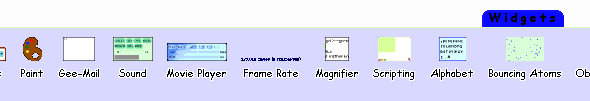
\includegraphics[scale=0.65]{Imatges/figura24-1}
\end{center}
\caption{Obriu la solapa dels \emph{widgets} per obtenir l'eina \emph{Paint}}
\label{fig2401}
\end{figure}

Utilitzant \emph{Paint}, dibuixeu un petit avió, com veieu a la figura~\ref{fig2402}. El nostre avió és una petita creu, però dibuixeu el vostre com us vingui de gust. Un cop heu acabat el dibuix, premeu el botó \emph{Keep}. L'editor de dibuixos desapareixerà, i a la pantalla quedarà un esbós (\emph{sketch}) que sembla un avió. L'avió que heu dibuixat s'anomena \emph{jugador} en l'argot eToy. \index{Paint, eina; obrir per dibuixar un avió}
\begin{figure}[h!]
\begin{center}
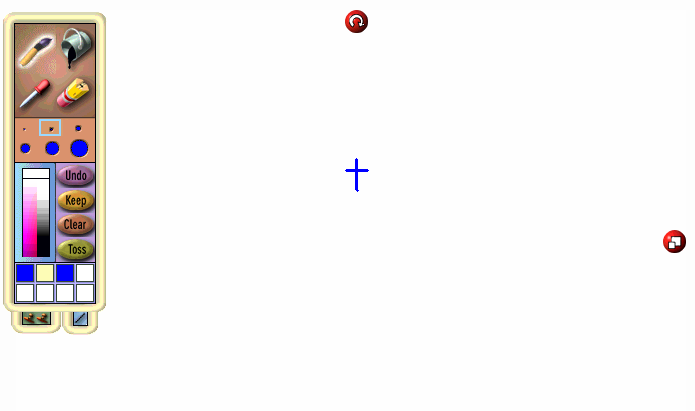
\includegraphics[scale=0.5]{Imatges/figura24-2}
\end{center}
\caption{Dibuixar un avió amb l'eina \emph{Paint}}
\label{fig2402}
\end{figure}

\subsection{Pas 2: Jugar amb l'halo}
\index{avió!jugar amb l'halo|(}
\index{nanses de l'halo, descripció de}
\index{halo de nanses!manipular per l'avió|(}
Ara, si feu clic sobre del vostre dibuix amb el botó dret del ratolí (o l'equivalent), veureu aparèixer un halo al voltant del dibuix, com es mostra a la figura~\ref{fig2403}. Cada nansa de l'halo té un color, una icona i una funció. Aquí les explicarem breument. Fixeu-vos que diferents tipus de dibuixos faran aparèixer diferents tipus de nanses. Podeu obtenir una descripció de la nansa aturant el ratolí al damunt durant un moment. 
\begin{figure}[h!]
\begin{center}
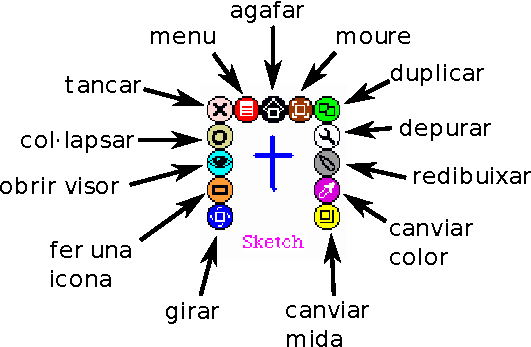
\includegraphics[scale=1]{Imatges/figura24-3}
\end{center}
\caption{Un halo envolta un dibuix}
\label{fig2403}
\end{figure}

\begin{itemize}
\item La nansa rosa amb una creu destrueix el dibuix. En funció de les preferències, el dibuix anirà a la paperera o serà completament eliminat. Si va a parar a la paperera, podeu recuperar-lo i tornar-lo a utilitzar.
\item La nansa vermella amb rectangles petits fa aparèixer el menú associat al dibuix. El menú depén del dibuix amb què esteu interaccionant. Proporciona moltes accions per manipular el dibuix.
\item La nansa negra selecciona el dibuix. Fixeu-vos que seleccionant un dibuix canvieu el seu \emph{contenidor}. Uilitzeu la nansa marró per moure el dibuix dins del contenidor. Utilitzeu la nansa vermella per inserir el dibuix dins del dibuix que té a sota. La idea és que podeu inserir un \emph{morph} dins del \emph{morph} que té a sota obrint la nansa vermella i seleccionant l'opció del menú \textbf{embed into}. Aquesta operació us ofereix un \emph{morph} on inserir el vostre \emph{morph}. Un cop ho heu fet, movent el \emph{morph} on heu inserit el vostre \emph{morph} es mouran els dos \emph{morphs}. Amb la nansa negre podeu ``des-inserir'' el vostre \emph{morph} del seu contenidor, mentre que amb la nansa marró, podeu moure el \emph{morph} només dins del contenidor.
\item La nansa marró amb un quadrat mou el dibuix sense canviar el seu contenidor.
\item La nansa verda amb dos quadrats duplica el dibuix.
\item La nansa gris amb una eina dibuixada ofereix possibilitats de depuració, que normalment són utilitzades per ``squeakers'' experts.
\item La nansa de color gris fosc té un llapis amb el qual podeu repintar el dibuix.
\item La nansa de color rosa fosc amb un comptagotes canvia el color del dibuix. No funciona amb dibuixos com el nostre avió. Per canviar el color d'un dibuix creat per vosaltres, necessiteu la nansa gris fosc. Si trieu aquesta nansa, tornareu a l'eina \emph{Paint}, on podeu fer qualsevol canvi sobre el vostre dibuix. La nansa rosa fosc és més apropiada per canviar els colors de les fonts, del rectangles o dels costats.
\item La nansa groga amb un quadrat i una barra canvia la mida del dibuix.
\item La nansa blava amb un quadrat petit serveix per girar el dibuix.
\item La nansa de color taronja amb un rectangle petit produeix una icona que representa l'objecte pel sistema d'icones d'eToy (més endavant explicarem més detalls).
\item La nansa cian amb un ull obre un \emph{visualitzador} (\emph{viewer}) per al dibuix. El visualitzador presenta una representació gràfica dels mètodes i les variables d'instància de l'objecte.
\item La nansa de color verd pàl·lid amb un cercle col·lapsa el dibuix.
\end{itemize}

Per programar dins l'entorn eToy utilitzem un visualitzador. Així, obriu un visualitzador de l'avió fent clic a la nansa cian amb un ull. Hauríeu d'obtenir les eines que podeu veure a la figura~\ref{fig2404} \index{eToy, sistema!obrir un visualitzador}
\begin{figure}[h!]
\begin{center}
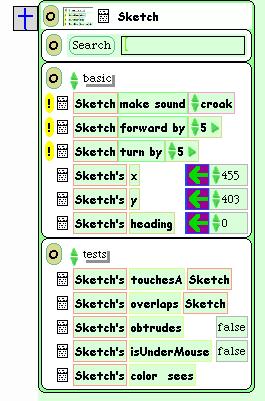
\includegraphics[scale=0.35]{Imatges/figura24-4}
\end{center}
\caption{Obrir un visualitzador}
\label{fig2404}
\index{visualitzador (\emph{viewer})!obrir dins eToy}
\end{figure}

La figura~\ref{fig2405} explica els principals components d'un visualitzador. A dalt de tot, el nom del dibuix (\emph{sketch}) pot ser modificat. \index{eToy, sistema!modificar noms dels dibuixos}Per defecte el vostre dibuix s'anomena \textsf{Sketch}. Us suggerim que l'anomeneu ``avió'' editant el nom al visualitzador A més de canviar el nom, podeu obrir un menú, com veieu a la figura. Amb aquest menú podeu afegir noves variables a l'objecte, obtenir un \emph{script} buit o aconseguir una icona representant l'objecte. \index{nom dels dibuixos, modificar a eToy}
\newpage
\begin{figure}
\begin{center}
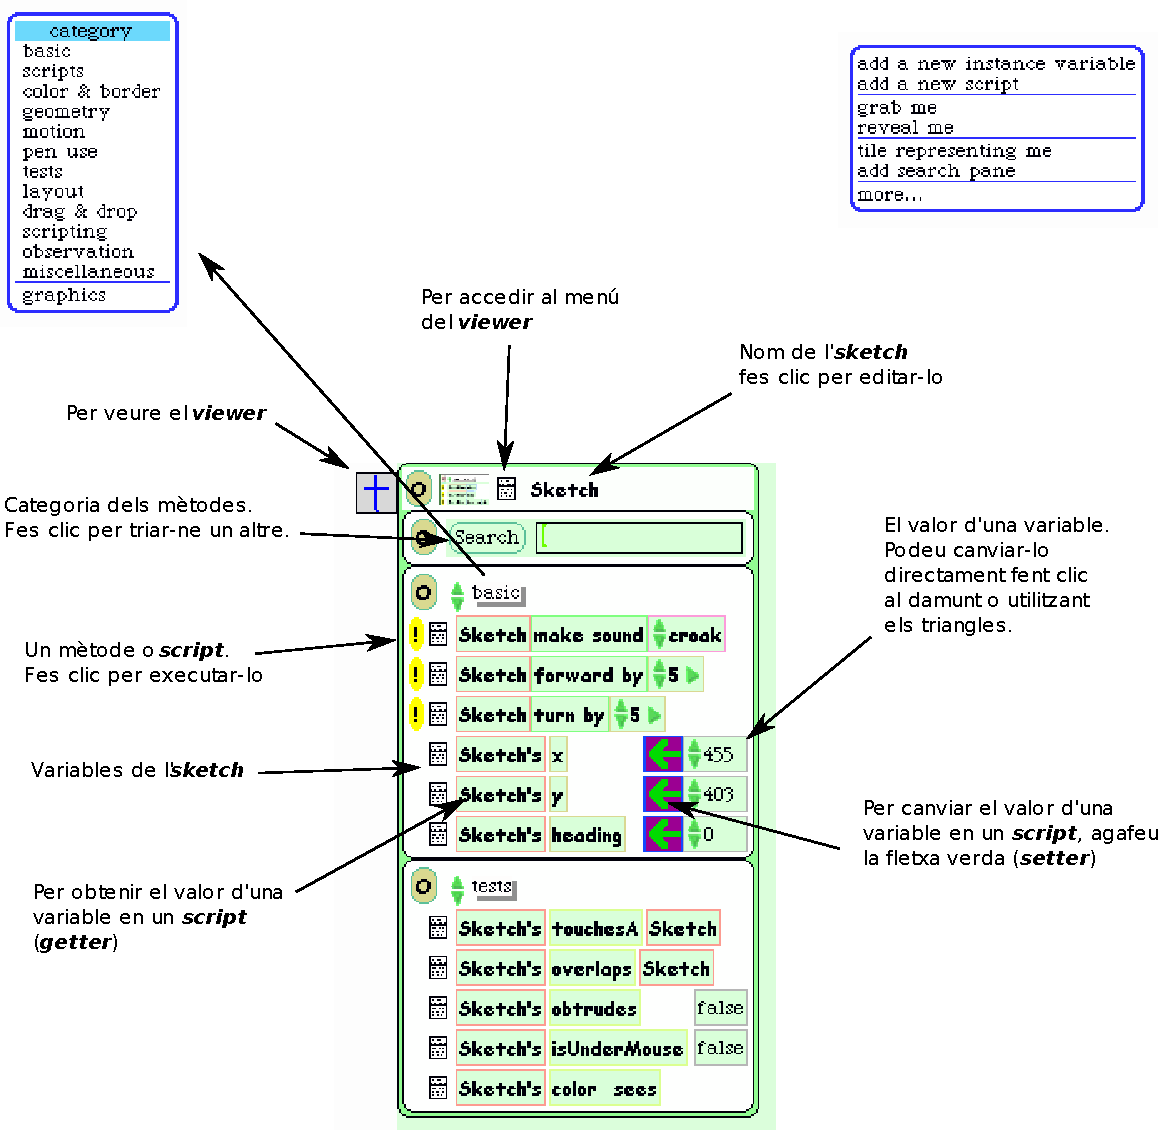
\includegraphics[scale=0.7]{Imatges/figura24-5}
\end{center}
\caption{Entendre un visualitzador}
\label{fig2405}
\index{visualitzador (\emph{viewer})!parts de}
\end{figure}
\newpage
Al visualitzador es mostren les categories. El nom d'una categria es mostra a la dreta de dos triangles verds que apunten amunt i avall. A la figura~\ref{fig2405} podeu veure les categories \textsf{basic} i \textsf{tests}. Podeu explorar-les utilitzant els petits triangles dobles. També podeu fer clic al mateix nom de la categoria per obtenir una llista de totes les categories.\index{categories!mostrar en el visualitzador d'eToy} \index{viewer@\emph{viewer}|see{visualitzador}} \index{visualitzador (\emph{viewer})!mostrar categories en el}

Sota cada categoria podeu veure una llista de mètodes. Quan un mètode pot ser executat, hi ha un signe d'admiració groc al costat. Premeu el signe d'admiració davant del mètode \textsf{forward} i veure l'avió movent-se cap endavant. Hi ha també mètodes que només accedeixen a o canvien el valor d'una variable. Anomenem a aquests mètodes \emph{d'accés}: són mètodes \emph{getter}, per accedir als valors, o mètodes \emph{setter} per modificar-los. \index{getter@\emph{getter}, mètodes; mostrar per a les categories a eToy} \index{setter@\emph{setter}, mètodes; mostrar per a les categories a eToy}\index{accés (mètodes de), mostrar per les categories en eToy} \index{valors!modificar els de les variables a eToy} \index{variables!modificar els valors a eToy}

Fixeu-vos que podeu modificar el valor d'una variable directament utilitzant els triangles de color verd, o escrivint un valor directament sobre la capsa de la variable. Proveu, per exemple, de canviar la variable \textsf{x} amb el valor \textsf{800}. Dins un \emph{script}, com que no podeu canviar interactivament el valor d'una variable, hauríeu d'utiltzar mètodes \emph{getter} i \emph{setter}. Podeu obtenir el mètode \emph{getter} per a la variable \textsf{x} arrosegant la capsa \textsf{x} a l'escriptori. Per obtenir el mètode \emph{setter}, hauríeu d'arrossegar la fletxa verda gran, com veieu a la figura~\ref{fig2406}.\index{metodes@mètodes!mostrar per a les categories d'eToy}
\begin{figure}[h!]
\begin{center}
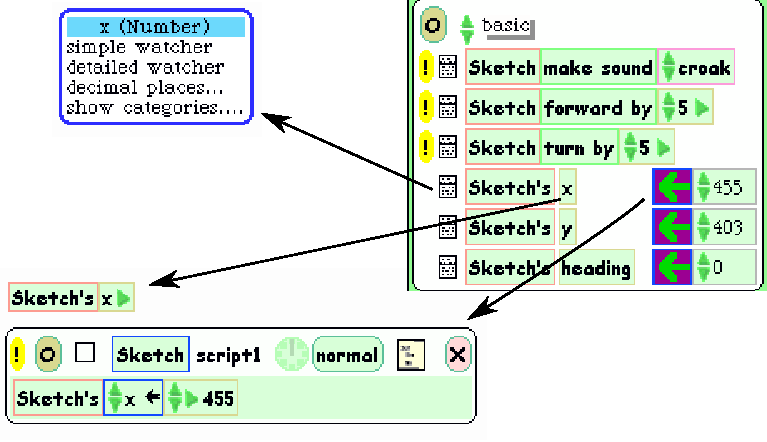
\includegraphics[scale=0.75]{Imatges/figura24-6}
\end{center}
\caption{Accedir a les variables dins d'un \emph{script}}
\label{fig2406}
\end{figure}

El nombre a la dreta de la fletxa verda gran és el valor de la variable. Si moveu l'avió utilitzant la nansa negra o marró, veureu les variables \textsf{x} i \textsf{y} canviar els seus valors.

També podeu tenir \emph{observadors} (\emph{watchers}), que proporcionen una manera d'espiar els valors de les variables. Per crear un observador, podeu fer clic a la icona petita de menú que hi ha a l'esquerra d'una variable del dibuix. Hauríeu d'obtenir el menú que veieu a la figura~\ref{fig2407}. Després podeu triar crear un observador senzill, que mostrarà només el valor d'una variable, o un observador detallat, que podeu utilitzar per canviar el valor d'una variable espiada.\index{eToy, sistema!utilitzar observadors} \index{observadors, utilitzar a eToy}
\begin{figure}[h!]
\begin{center}
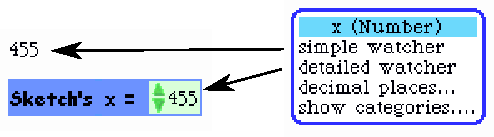
\includegraphics[scale=1]{Imatges/figura24-7}
\end{center}
\caption{Els observadors: Espiar les vostres variables}
\label{fig2407}
\end{figure}

\subsection{Pas 3: Arrossegar i deixar un mètode per crear nous \emph{scripts}}
\index{avió!arrossegar i deixar un mètode per crear nous \emph{scripts}}
\index{scripts@\emph{scripts}!crear per a l'avió}
\index{metodes@mètodes!arrossegar i deixar anar per crear nous \emph{scripts} per a l'avió}
\index{eToy, sistema!crear nous \emph{scripts} amb}
Si preneu un mètode com \textsf{forward by} del visualitzador i el deixeu sobre l'escriptori, ja teniu un \emph{script}. Hauríeu d'obtenir, per exemple, l'\emph{script} que veieu a la figura~\ref{fig2408}.
\newpage
\begin{figure}[h!]
\begin{center}
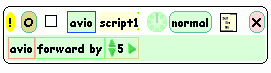
\includegraphics[scale=0.8]{Imatges/figura24-8}
\end{center}
\caption{Creem un \emph{script}}
\label{fig2408}
\end{figure}

\begin{figure}[h!]
\begin{center}
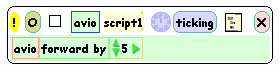
\includegraphics[scale=0.8]{Imatges/figura24-9}
\end{center}
\caption{Quan el rellotge està en marxa, l'\emph{script} s'està executant}
\label{fig2409}
\end{figure}

\begin{figure}[h!]
\begin{center}
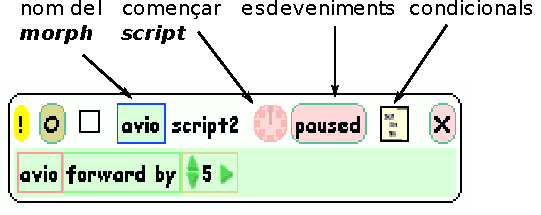
\includegraphics[scale=1]{Imatges/figura24-10}
\end{center}
\caption{Les diferents parts d'un \emph{script}}
\label{fig2410}
\end{figure}
\newpage
Per executar l'\emph{script} només cal que feu clic sobre la icona del rellotge. El rellotge es posa en marxa (estat \emph{ticking}, veure figura~\ref{fig2409}), la qual cosa vol dir que el vostre \emph{script} s'executa a intervals de temps regulars.

La figura~\ref{fig2410} mostra les diferents parts d'un \emph{script}: podeu veure el nom del dibuix, el nom de l'\emph{script}, un rellotge per començar i aturar l'execució de l'\emph{script}, una llista d'esdeveniments als quals pot enllaçar-se un \emph{script}, i la creació d'un condicional, o \emph{test}.\index{avió!jugar amb l'halo|)}

\subsection{Pas 4: Afegir mètodes}
\index{avió!afegir mètodes|(}
\index{halo de nanses!manipular per l'avió|)}
\index{metodes@mètodes!afegir per a l'avió|(}
Quan executeu l'\emph{script}, podeu veure que l'avió vola en línia recta. Sens dubte voldríeu que el vostre avió fos capaç de girar. Per aconseguir això, us cal afeir mètodes a l'\emph{script}. Arrossegueu el mètode \textsf{turn by} del visualitzador i deixeu-lo anar dins de l'\emph{script}. L'\emph{script} us hauria de mostrar el lloc on quedarà el nou mètode quan el deixeu anar, ensenyant-vos unes capses de color verd. Deixeu anar el mètode en una de les capses. Hauríeu d'obtenir un \emph{script} similar al que veieu a la figura~\ref{fig2411}. \index{turn: mètode!afegir per a un avió}
\begin{figure}[h!]
\begin{center}
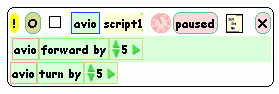
\includegraphics[scale=1]{Imatges/figura24-11}
\end{center}
\caption{El mètode \textsf{\upshape turn by} ha estat afegit a l'\emph{script}}
\label{fig2411}
\end{figure}

Ara, quan executeu l'\emph{script}, l'avió hauria de girar en un cercle. De fet, un dibuix és similar a un robot, i podeu veure el que l'avió està fent dient-li que baixi el llapis. Per fer això, busqueu la variable \textsf{penDown} dins del visualitzador i poseu el seu valor a \textsf{true}, com a l'\emph{script} que veieu a la figura~\ref{fig2412}. El resultat es mostra a la figura~\ref{fig2413}.\index{avió!volar} \index{traces!fer que l'avió dibuixi}
\begin{figure}[h!]
\begin{center}
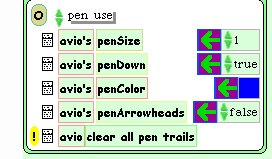
\includegraphics[scale=0.6]{Imatges/figura24-12}
\end{center}
\caption{Un cop el llapis és avall, l'avió dibuixarà una traça a l'escriptori, com veieu a la figura~\ref{fig2413}.}
\label{fig2412}
\end{figure}

\begin{figure}[h!]
\begin{center}
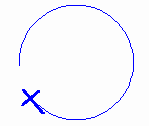
\includegraphics[scale=0.75]{Imatges/figura24-13}
\end{center}
\caption{L'avió ha baixat el seu llapis, i podem veure que vola en un cercle.}
\label{fig2413}
\end{figure}

Fixeu-vos que podeu triar quan s'executarà l'\emph{script} utilitzant el botó d'esdeveniments a l'\emph{script}. La figura~\ref{fig2414} mostra tots els esdeveniments que podeu fer servir. Obtindreu aquest menú fent clic dins el text a la dreta del rellotge.\index{avió!afegir mètodes|)}\index{eToy, sistema!mostrar el menú d'esdeveniments}\index{esdeveniments, menú; mostrar dins el sistema eToy}
\begin{figure}[h!]
\begin{center}
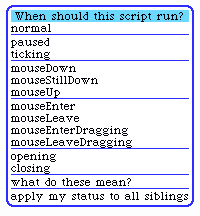
\includegraphics[scale=0.6]{Imatges/figura24-14}
\end{center}
\caption{Una llista d'esdeveniments disponibles.}
\label{fig2414}
\end{figure}

\section{\emph{Joysticks} en acció}
\index{metodes@mètodes!afegir per a l'avió|)}
\index{avió!crear \emph{joystick} per|(}
Volar en cercles és divertit, però probablement us agradaria conduir el vostre avió. Podeu variar l'angle de gir de l'avió, en lloc de girar sempre el mateix angle, associant-lo a l'estat d'un \emph{joystick}.\index{eToy, sistema!exemple pilotant un avió|)}
\index{eToy, sistema!utilitzar \emph{joystick} per l'exemple de l'avió|(}

\subsection{Pas 1: Crear un \emph{joystick}}
\index{joystick@\emph{joystick}!crear per a un avió}
Primer creeu el \emph{joystick} arrossegant-ne un de la solapa \emph{supplies} i deixant-lo anar a sobre de l'escriptori. El cercle vermell representa el capdamunt del \emph{joystick} (figura~\ref{fig2415}), i amb ell podeu indicar quina direcció i quina quantitat d'energia volem posar en el moviment de l'avió.
\begin{figure}[h!]
\begin{center}
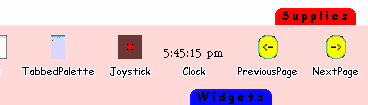
\includegraphics[scale=0.75]{Imatges/figura24-15}
\end{center}
\caption{Crear un \emph{joystick}.}
\label{fig2415}
\end{figure}

\subsection{Pas 2: Experimentar amb un \emph{joystick}}
\index{avió!experimentar amb el \emph{joystick}}
\index{joystick@\emph{joystick}!experimentar amb}
\index{metodes@mètodes!mostrar pel \emph{joystick} de l'avió}
Segon, obriu el visualitzador del \emph{joystick} utilitzant la nansa apropiada. Després, explorant els mètodes, en trobareu alguns d'útils sota la categoria \textsf{joystick} (figura~\ref{fig2416}). Feu moviments amb el \emph{joystick} i observeu les variables. La variable \textsf{amount} representa la quantitat d'energia invertida en el moviment; és a dir, podeu triar a més de la direcció en què es mou el \emph{joystick}, la força del moviment. La variable \textsf{angle} representa la direcció en la qual esteu movent el \emph{joystick}, i us deixarem endevinar el que representen les altres dues variables.
\begin{figure}[h!]
\begin{center}
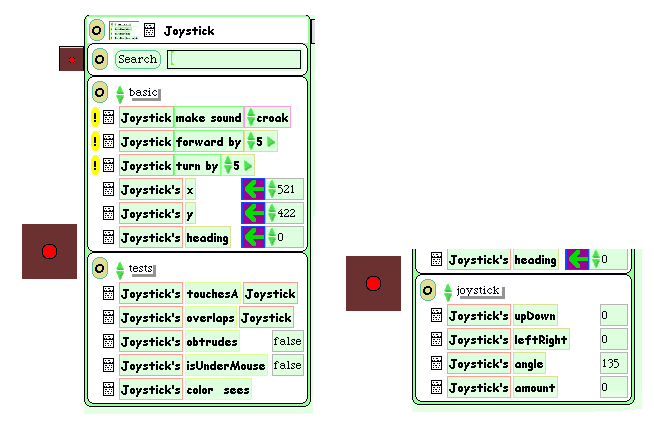
\includegraphics[scale=2]{Imatges/figura24-16}
\end{center}
\caption{Mètodes sota la categoria \textsf{\upshape joystick}.}
\label{fig2416}
\end{figure}

\subsection{Pas 3: Vincular el \emph{joystick} i l'\emph{script}}
\index{joystick@\emph{joystick}!vincular a un \emph{script}|(}
\index{scripts@\emph{scripts}!vincular el \emph{joystick} de l'avió amb|(}
Per poder conduir l'avió, heu de canviar el valor del mètode \textsf{turn by} a l'\emph{script} pel valor donat pel \emph{joystick}. Per a això, la variable \textsf{leftRight} sembla ser la que necessitem. Arrossegueu la variable directament sobre l'argument del mètode \textsf{turn by} a l'\emph{script}. Pot costar-li un moment acceptar la variable, però hauríeu d'aconseguir l'\emph{script} de la figura~\ref{fig2417}.
\begin{figure}[h!]
\begin{center}
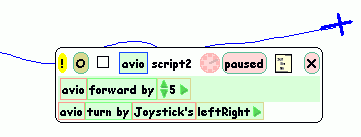
\includegraphics[scale=0.75]{Imatges/figura24-17}
\end{center}
\caption{Ara, la variable del \emph{joystick} \textsf{\upshape leftRight} controlarà el gir de l'avió.}
\label{fig2417}
\end{figure}

Ara feu clic sobre el rellotge i conduïu el vostre avió amb el \emph{joystick}. Com podeu veure, si controléssim la velocitat de l'avió en milloraríem la conducció. Proveu de trobar-hi una solució. Considereu la variable \textsf{amount}; us pot ajudar.\index{avió!crear \emph{joystick} per|)} \index{eToy, sistema!utilitzar \emph{joystick} per l'exemple de l'avió|)} \index{joystick@\emph{joystick}!vincular a un \emph{script}|)} \index{scripts@\emph{scripts}!vincular el \emph{joystick} de l'avió amb|)}

\section{Crear una animació}
\index{eToy, sistema!crear animacions a|(}
La idea per crear una animació és la següent: primer dibuixeu els marcs individuals de l'animació i els poseu en un contenidor d'animacions. Després creeu un dibuix senzill, la representació gràfica del qual serà sustituïda pels elements de l'animació. Per fer això podeu escriure un \emph{script} que fa que el dibuix sembli els diferents marcs que hi ha al contenidor.

\subsection{Pas 1: Crear el contenidor}
\index{animacions!crear contenidors per a}
\index{contenidors!crear per a animacions}
Per crear una animació, heu de crear un contenidor (\emph{Holder}). Un contenidor és un objecte gràfic que pot contenir altres objectes gràfics. També sap quin és l'objecte seleccionat d'entre tots els que conté. Per crear un contenidor, arrossegueu-lo de la solapa anomenada \emph{supplies} (figura~\ref{fig2418} i deixeu-lo anar sobre l'escriptori.
\begin{figure}[h!]
\begin{center}
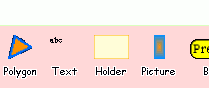
\includegraphics[scale=1]{Imatges/figura24-18}
\end{center}
\caption{Podem fer servir la solapa vermella per crear un contenidor.}
\label{fig2418}
\end{figure}

Es crea un contenidor buit (figura~\ref{fig2419}).
\begin{figure}[h!]
\begin{center}
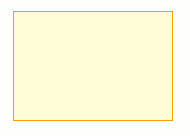
\includegraphics[scale=0.5]{Imatges/figura24-19}
\end{center}
\caption{Un contenidor buit.}
\label{fig2419}
\end{figure}

\subsection{Pas 2: Dibuixar els elements de l'animació}
\index{elements de l'animació!dibuixar}
\index{dibuixar!elements de l'animació}
Pel segon pas, hauríeu de dibuixar allò que vulgueu animar utilitzant l'editor de dibuixos \emph{Paint} que ja hem vist abans. Us recomanem que primer feu un dibuix, i el dupliqueu amb la nansa verda. Després seleccioneu la nansa gris fosc per redibuixar el que heu fet. D'aquesta manera, podeu crear diversos dibuixos modifcant-ne un pas a pas. Ara pintarem un cuc en dues posicions diferents (figura~\ref{fig2420}).\index{cuc, animar}
\begin{figure}[h!]
\begin{center}

\includegraphics[scale=0.6]{Imatges/figura24-20}
\end{center}
\caption{Un cuc en dues posicions diferents.}
\label{fig2420}
\end{figure}
\begin{figure}[h!]
\begin{center}
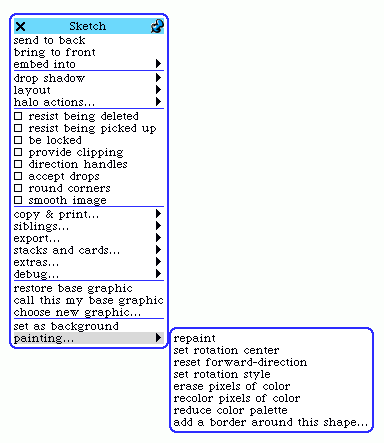
\includegraphics[scale=0.4]{Imatges/figura24-21}
\end{center}
\caption{El menú de pintar de la nansa vermella.}
\label{fig2421}
\end{figure}

Fixeu-vos que també podeu utilitzar l'opció de pintar del menú de la nansa vermella (figura~\ref{fig2421}), però us suggerim que utilizeu les nanses proporcionades tant com us sigui possible. \index{pintar amb la nansa vermella, utilitzar en animacions}

\subsection{Pas 3: Deixar els dibuixos dins del contenidor}
\index{contenidors!deixar els dibuixos dins del}
\index{dibuixos, deixar-los dins de contenidors}
\index{contenidors de dibuixos, crear per les animacions d'eToy}
El proper pas és simplement posar els dibuixos dins del contenidor. Un rectangle negre (figura~\ref{fig2422}) representa el dibuix actualment seleccionat dins del contenidor.
\begin{figure}[h!]
\begin{center}
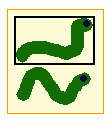
\includegraphics[scale=0.75]{Imatges/figura24-22}
\end{center}
\caption{El cuc del rectangle negre és el dibuix seleccionat.}
\label{fig2422}
\end{figure}

\subsection{Pas 4: Crear un dibuix senzill com a base de l'animació}
\index{animacions!crear dibuixos senzills com a base de}
\index{visualitzador (\emph{viewer})!de la base de l'animació}
Ara us cal un dibuix que s'utilitzarà com a receptacle de l'animació. Per tant, hauríeu de crear un dibuix senzill, com una el·lipse, que agafareu i arrossegareu de la solapa \emph{supplies}. Obriu després un visualitzador d'aquest dibuix, com veieu a la figura~\ref{fig2423}.
\begin{figure}[h!]
\begin{center}
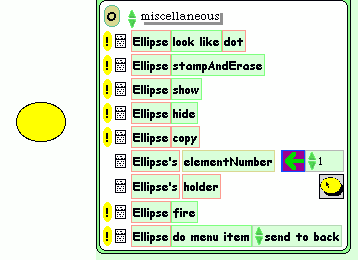
\includegraphics[scale=0.5]{Imatges/figura24-23}
\end{center}
\caption{Un visualitzador del receptacle del dibuix.}
\label{fig2423}
\end{figure}

\subsection{Pas 5: Crear un \emph{script} amb \textsf{lookLike}}
\index{lookLike mètode, crear \emph{scripts} amb}
\index{scripts@\emph{scripts}!crear amb el mètode lookLike}
A partir del dibuix senzill, aquí l'el·lipse, podeu crear un nou \emph{script} arrossegant el mètode \textsf{lookLike dot} (mostrat a la figura~\ref{fig2423} del visualitzador a l'escriptori. Aquesta acció hauria d'haver creat l'\emph{script} descrit a la figura~\ref{fig2424}.
\begin{figure}[h!]
\begin{center}
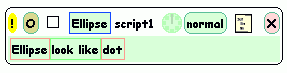
\includegraphics[scale=0.75]{Imatges/figura24-24}
\end{center}
\caption{Un \emph{script} amb \textsf{\upshape lookLike dot}}
\label{fig2424}
\end{figure}

\subsection{Pas 6: Mostrar l'element seleccionat de l'animació}
\index{elements de l'animació!mostrar|(}
\index{contenidors!obrir dins del visualitzador}
Ara hauríeu d'indicar que l'el·lipse s'hauria d'assemblar a l'element actualment seleccionat del contenidor. Seleccioneu el contenidor i obriu-lo en un visualitzador, com veieu a la figura~\ref{fig2425}. \index{visualitzador (\emph{viewer})!obrir un contenidor en un}
\begin{figure}[h!]
\begin{center}
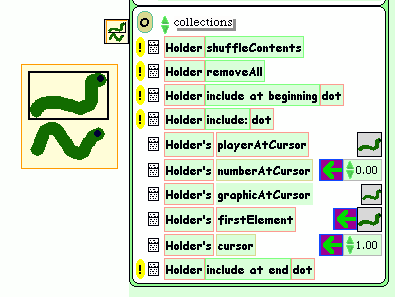
\includegraphics[scale=0.5]{Imatges/figura24-25}
\end{center}
\caption{El contenidor obert en un visualitzador.}
\label{fig2425}
\end{figure}

Busqueu la categoria \textsf{collection} triant ``\textsf{basic}'', com veieu a la figura~\ref{fig2426}.\index{basic (botó), prémer a eToy} \index{collection categoria, buscar} \index{eToy, sistema!botó basic|(}
\begin{figure}[h!]
\begin{center}
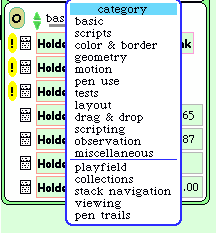
\includegraphics[scale=0.5]{Imatges/figura24-26}
\end{center}
\caption{Prement el botó ``\textsf{\upshape basic}'' us permet accedir a \textsf{\upshape collection}.}
\label{fig2426}
\end{figure}

De la llista de mètodes arrossegueu el mètode anomenat \textsf{playerAtCursor}, que retorna el jugador, és a dir, l'element gràfic dins el contenidor que és a la posició actual. Deixeu-lo anar dins del quadrat amb un punt al mig (aquesta capsa representa l'argument del mètode \textsf{lookLike}). Obtindreu l'\emph{script} de la figura~\ref{fig2427}. \index{elipses@el·lipses!canviar l'aparença a eToy} \index{eToy, sistema!botó basic|)}\index{playerAtCursor mètode, arrossegant a eToy}
\begin{figure}[h!]
\begin{center}
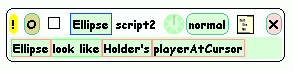
\includegraphics[scale=0.6]{Imatges/figura24-27}
\end{center}
\caption{Ara l'el·lipse hauria de tenir l'aparença de l'element apuntat pel cursor.}
\label{fig2427}
\end{figure}

\subsection{Pas 7: Canviar l'element seleccionat d'un contenidor}
\index{elements de l'animació!mostrar|)}
\index{eToy, sistema!canviar els elements d'un contenidor|(}
\index{contenidor, elements de; canviar a eToy|(}
Si executeu l'\emph{script} previ utilitzant el botó \emph{ticking}, l'\emph{script} canviarà la forma de l'el·lipse per l'element gràfic actualment seleccionat. Encara, però, no tenim cap animació. Per a això, ens cal trobar una manera de canviar l'element seleccionat actualment d'un contenidor. De fet, un contenidor té un índex, anomenat \textsf{cursor}, que representa el nombre associat a l'element seleccionat. N'hi ha prou amb incrementar aquest índex per fer que el contenidor seleccioni un altre element gràfic.

Per canviar el valor de la variable anomenada \textsf{cursor}, arrossegueu la fletxa (mostrada a la dreta de la figura~\ref{fig2428}) i poseu-la a la línia següent de l'\emph{script} que ja hem vist. Obtindreu l'\emph{script} de la figura~\ref{fig2429}, que diu que la variable conté el valor 1.\index{assignació, introduir a eToy}
\begin{figure}[h!]
\begin{center}
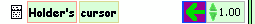
\includegraphics[scale=0.75]{Imatges/figura24-28}
\end{center}
\caption{El cursor dins el jugador.}
\label{fig2428}
\end{figure}
\begin{figure}[h!]
\begin{center}
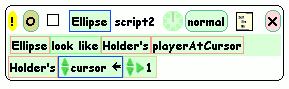
\includegraphics[scale=0.6]{Imatges/figura24-29}
\end{center}
\caption{Introduir una assignació.}
\label{fig2429}
\end{figure}

Ara, si feu clic als triangles dobles de color verd del \emph{setter} a l'\emph{script}, veureu que podeu incrementar el valor del cursor en una certa quantitat (figura~\ref{fig2430}). Ara l'animació hauria de funcionar.\index{eToy, sistema!canviar els elements d'un contenidor|)}
\begin{figure}[h!]
\begin{center}
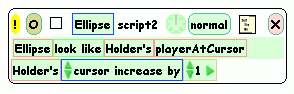
\includegraphics[scale=0.6]{Imatges/figura24-30}
\end{center}
\caption{Incrementar el cursor.}
\label{fig2430}
\end{figure}

\subsection{Una altra manera}
\index{cursor, canviar a eToy el valor del}
\index{contenidor, elements de; canviar a eToy|)}
Per aconseguir el mateix efecte, podeu simular l'expressió \textsf{cursor := cursor + 1}, que mourà el cursor al proper element. Per tant, arrossegueu la part esquerra del cursor  des del visualitzador fins el lloc de l'1 a l'\emph{script}, i obtindreu l'\emph{script} de la figura~\ref{fig2431}.
\begin{figure}[h!]
\begin{center}
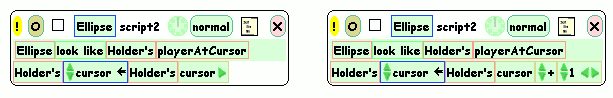
\includegraphics[scale=0.6]{Imatges/figura24-31}
\end{center}
\caption{Utilitzar l'expressió \textsf{\upshape cursor := cursor + 1}.}
\label{fig2431}
\end{figure}

Ara només us cal fer clic al triangle verd i petit al final de la capsa del cursor a l'\emph{script} per fer aparèixer l'expressió \textsf{+ 1}, com es veu en l'\emph{script} final. La primera solució, però, és més senzilla.

Us recomanem que els lectors interessats a utilitzar eToy a classe llegiu el llibre esmentat al principi del capítol. Presenta molts aspectes pedagògics que poden utilitzar-se amb aquest exemple.\index{eToy, sistema!crear animacions a|)}

\section{Cotxes i conductors}
\index{eToy, sistema!cotxes i conductors, exemple|(}
Ara ens agradaria ensenyar-vos com podeu construir un \emph{script} per controlar un cotxe amb un volant. Aquest exercici pot ser útil als mestres per ensenyar l'ús de la divisió com a desmultiplicador, tal com es fa en cotxes reals, però també es pot fer servir per diversió.

\subsection{Pas 1: Dibuixar un cotxe i un volant}
\index{cotxe!dibuixar a eToy}
\index{volant!dibuixar a eToy}
Utilitzant l'editor de dibuixos, dibuixeu un cotxe i un volant, com els de la figura~\ref{fig2432}.
\begin{figure}[h!]
\begin{center}

\includegraphics[scale=0.75]{Imatges/figura24-32}
\end{center}
\caption{Dibuixeu un cotxe i un volant.}
\label{fig2432}
\end{figure}

\subsection{Pas 2: Girar el cotxe en un cercle}
\index{cotxe!girar en cercles a eToy}
Obriu un visualitzador per al cotxe, canvieu-li el nom pel de ``cotxe'' i arrossegueu i deixeu anar el mètode \textsf{forward by} tal com ja heu fet abans. S'hauria d'obtenir l'\emph{script} mostrat a la figura~\ref{fig2433}.\index{forward mètode, arrossegar i deixar a eToy}
\begin{figure}[h!]
\begin{center}
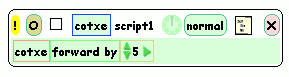
\includegraphics[scale=0.6]{Imatges/figura24-33}
\end{center}
\caption{Arrossegueu i deixeu anar el mètode \textsf{\upshape forward}.}
\label{fig2433}
\end{figure}

Després arrossegueu i deixeu anar el mètode \textsf{turn} sota el mètode anterior a l'\emph{script} que acabeu de crear. Hauríeu de tenir l'\emph{script} de la figura~\ref{fig2434}, que quan s'executa fa que el cotxe doni voltes en un cercle.\index{turn: mètode!arrossegar i deixar a eToy}
\begin{figure}[h!]
\begin{center}
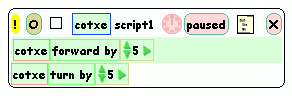
\includegraphics[scale=0.6]{Imatges/figura24-34}
\end{center}
\caption{Arrossegueu i deixeu anar el mètode \textsf{\upshape turn}.}
\label{fig2434}
\end{figure}

\subsection{Pas 3: Utilitzar la direcció del volant}
\index{volant!utilitzar la direcció del|(}
\index{angles!vincular amb la posició del volant a eToy|(}
\index{posició!vincular amb l'angle del volant a eToy|(}
\index{rotació, determinar pel volant d'eToy|(}
Ara heu de vincular l'angle que gira el cotxe amb la posició del volant. Hem de trobar una manera de girar el volant i determinar quina quantitat ha girat. El primer problema és fàcil de resoldre: feu aparèixer l'halo, feu clic sobre la nansa blava i gireu (figura~\ref{fig2435}). Això fa que giri el volant. Per resoldre el segon problema, obriu un visualitzador del volant, canvieu-li el nom per ``volant'', i busqueu la variable \textsf{heading} dins el visualitzador (l'expressió serà \textsf{volant's heading}). Quan gireu el volant amb la nansa, el valor de la variable canvia. Aquesta variable representa l'angle de rotació respecte del dibuix original.\index{halo de nanses!per conduir el volant a eToy} \index{heading@\emph{heading} valor, per conduir el volant a eToy}
\begin{figure}[h!]
\begin{center}
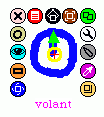
\includegraphics[scale=0.8]{Imatges/figura24-35}
\end{center}
\caption{El volant amb el seu halo de nanses.}
\label{fig2435}
\end{figure}

Ara que ja teniu totes les peces del trencaclosques, heu de dir-li al cotxe que giri no una quantitat determinada, sinó el que digui la direcció del volant.
Per fer això, arrossegueu l'expressió \textsf{volant's heading} des del visualitzador fins al nombre \textsf{5}, argument del mètode \textsf{turn} de l'\emph{script} anterior. hauríeu de tenir l'\emph{script} de la figura~\ref{fig2436}.
\begin{figure}[h!]
\begin{center}
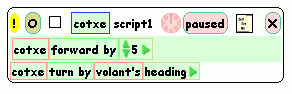
\includegraphics[scale=0.6]{Imatges/figura24-36}
\end{center}
\caption{Ara ja podem girar el cotxe amb el volant.}
\label{fig2436}
\end{figure}

Si fem clic sobre el petit rellotge de l'\emph{script}, el cotxe corre i podem controlar-lo des de la nansa blava de l'halo del volant. Us adoneu, però, que el seguiment no és perfecte. Els mestres haurien de proposar que els estudiants analitzessin el problema i suggerissin solucions.

La qüestió és que el valor de la direcció del volant s'hauria de dividir de manera que l'usuari pogués tenir un control més precís sobre el gir. Per fer-ho, feu clic sobre el petit triangle verd de més a la dreta dins del bloc de direcció del volant. Això afegeix més capses. Feu clic per triar la divisió $//$. Ara teniu un \emph{script} similar al de la figura~\ref{fig2437}.\index{// (divisió), triar per conduir el volant d'eToy} \index{divisió (//), triar per conduir el volant d'eToy} 
\begin{figure}[h!]
\begin{center}
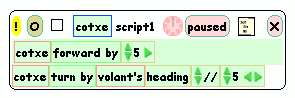
\includegraphics[scale=0.6]{Imatges/figura24-37}
\end{center}
\caption{Dividint el valor de la direcció del volant aconseguim un control més precís.}
\label{fig2437}
\end{figure}

El cotxe, el volant i els halos apareixen tots a la figura~\ref{fig2438}. Divertiu-vos controlant el cotxe!
\begin{figure}[h!]
\begin{center}
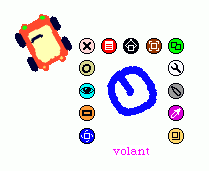
\includegraphics[scale=0.8]{Imatges/figura24-38}
\end{center}
\caption{Divertiu-vos amb el cotxe!}
\label{fig2438}
\end{figure}

Ara voldríem programar el cotxe de manera que pugui anar sol, automàticament, per una carretera. La idea és 
equipar al cotxe amb sensors que li diguin si marxa de la carretera. Un cop el cotxe hagi estat equipat amb sensors i convenientment programat, el posarem en una carretera, a veure què tal la segueix.  \index{rotació, determinar pel volant d'eToy|)}

No us mostrarem una solució completa d'aquest problema ja que pensem que us agradarà experimentar vosaltres mateixos. És més, la nostra solució no funciona gaire bé.\index{angles!vincular amb la posició del volant a eToy|)} \index{posició!vincular amb l'angle del volant a eToy|)}\index{volant!utilitzar la direcció del|)}

\subsection{Pas 1: Sensors}
\index{cotxe!afegir sensors a}
\index{sensors pel cotxe, crear a eToy}
\index{eToy, sistema!crear sensors}
A eToy podeu preguntar si un determinat color d'un dibuix pot veure un altre color que tingui a sota. Aquesta possibilitat pot ser utilitzada per construir un sensor. Un sensor serà un simple punt d'un color que li dirà al cotxe si està passant per sobre d'un altre color. Per equipar el vostre cotxe amb sensors, redibuixeu el cotxe i afegiu dos punts de colors, com veieu a la figura~\ref{fig2439}.
\begin{figure}[h!]
\begin{center}
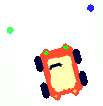
\includegraphics[scale=0.8]{Imatges/figura24-39}
\end{center}
\caption{Hem afegit dos sensors al cotxe.}
\label{fig2439}
\end{figure}

\subsection{Pas 2: La carretera}
\index{carretera!crear a eToy}
Utilitzant l'editor de dibuixos, feu una carretera d'un sol color. Després podeu provar de posar-hi diverses bandes de colors.\index{eToy, sistema!crear una carretera}
\begin{figure}[h!]
\begin{center}

\includegraphics[scale=0.2]{Imatges/figura24-40}
\end{center}
\caption{La carretera.}
\label{fig2440}
\end{figure}

\subsection{Pas 3: Condicions i tests a eToy}
\index{cotxe!expressar diferents comportaments per}
\index{eToy, sistema!condicions i tests a|(}
Obriu el visualitzador del  cotxe i arrossegueu i deixeu anar el mètode \textsf{forward by} sobre l'escriptori. Això crea un \emph{script} com aquells que ja esteu acostumats a crear.

Ara necessiteu una manera d'expressar diferents tipus de comportament en funció del valor del sensor. Per a això, hauríeu de poder expressar una condició, o test. Per obtenir un test, hauríeu d'arrosseguar el quadrat petit (segona capsa per la dreta al capdamunt de l'\emph{script}, prop del botó amb una creu), com veieu a la figura~\ref{fig2441}. Arrossegueu i deixeu anar aquesta petita icona de test dins de l'\emph{script}. Hauríeu d'aconseguir un \emph{script} similar al de la figura.
\begin{figure}[h!]
\begin{center}
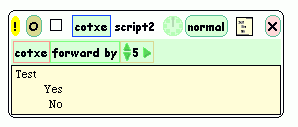
\includegraphics[scale=0.6]{Imatges/figura24-41}
\end{center}
\caption{Afegir un test a l'\emph{script}.}
\label{fig2441}
\end{figure}

Ara us cal trobar una manera d'activar els vostres sensors. Trobeu el mètode \textsf{color sees} a la categoria \textsf{test}, com veieu a la figura~\ref{fig2442}. Aquest mètode retorna \textsf{true} o \textsf{false} en funció de si una part del dibuix d'un determinat color passa sobre un altre color.
\begin{figure}[h!]
\begin{center}
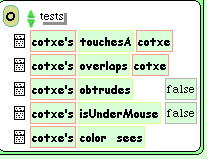
\includegraphics[scale=0.8]{Imatges/figura24-42}
\end{center}
\caption{Afegir un test a l'\emph{script}.}
\label{fig2442}
\end{figure}

Arrossegueu el mètode \textsf{color sees} dins de l'\emph{script} al costat de la paraula \textsf{Test}. Hauríeu d'obtenir un \emph{script} com el de la figura~\ref{fig2443}.
\index{eToy, sistema!condicions i tests a|)}
\begin{figure}[h!]
\begin{center}
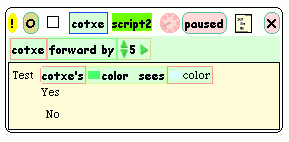
\includegraphics[scale=0.6]{Imatges/figura24-43}
\end{center}
\caption{Afegir un mètode \textsf{\upshape color sees} a l'\emph{script}.}
\label{fig2443}
\end{figure}

\subsection{Pas 4: Personalitzar els tests basats en colors}
\index{carretera!acolorir a eToy}
\index{color sees mètode, triar color en l'exemple del cotxe}
\index{color (tests), personalitzar}
\index{eToy, sistema!personalitzar tests basats en colors}
Com definirem el color que hauria d'utilitzar el test? És fàcil. Només cal que feu clic al damunt del quadradet de color dins del mètode \textsf{color sees}. Això obre automàticament un triador de color (figura~\ref{fig2444}). Amb el  triador de color, podeu triar el color d'un sensor. El primer color de l'\emph{script} hauria de canviar per reflectir aquesta tria de color. Feu la mateixa operació per a la segona capsa de color, però aquest cop trieu el color de la carretera (figura~\ref{fig2445}).
\begin{figure}[h!]
\begin{center}
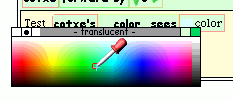
\includegraphics[scale=0.8]{Imatges/figura24-44}
\end{center}
\caption{Utilitzar el triador de color.}
\label{fig2444}
\end{figure}
\begin{figure}[h!]
\begin{center}
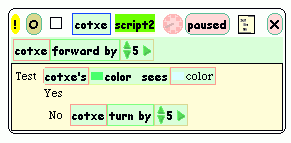
\includegraphics[scale=0.6]{Imatges/figura24-45}
\end{center}
\caption{Trieu el color de la carretera pel color que el cotxe veu.}
\label{fig2445}
\end{figure}

\subsection{Pas 5: Afegir accions}
\index{accions!afegir per a un cotxe a eToy}
\index{cotxe!afegir accions per a }
Ara podeu especificar que el cotxe hauria de girar quan el sensor no vegi el color de la carretera. Només cal que arrossegueu i deixeu anar el mètode \textsf{turn by} al costat de la paraula \textsf{No} a l'\emph{script}. Ara podeu seleccionar el cotxe, posar-lo a la carretera i prémer el rellotge per executar l'\emph{script}. Veieu la figura~\ref{fig2446}.
\begin{figure}[h!]
\begin{center}
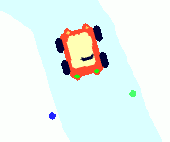
\includegraphics[scale=0.8]{Imatges/figura24-46}
\end{center}
\caption{El cotxe segueix la carretera!}
\label{fig2446}
\end{figure}

És clar que el comportament del cotxe no és perfecte, i us deixem a vosaltres la possibilitat de canviar-lo o de trobar una solució pròpia. \index{eToy, sistema!cotxes i conductors, exemple|)}

\section{Alguns trucs}
\index{eToy, sistema!personalitzar|(}
Ens agradaria ensenyar-vos alguns aspectes d'eToy que us poden ajudar. L'entorn eToy pot ser personalitzat, així que obriu el menú \textbf{playfield options\dots} (figura~\ref{fig2447}), deixeu que el ratolí s'aturi sobre les diferents opcions i llegiu-vos la bafarada d'ajuda. Algunes de les coses que podeu fer són:\index{playfield options menú, mostrar a eToy}
\begin{figure}[h!]
\begin{center}
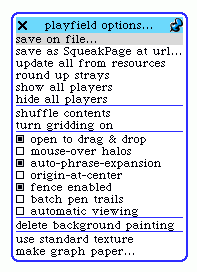
\includegraphics[scale=0.5]{Imatges/figura24-47}
\end{center}
\caption{El menú \textbf{playfield options\dots}}
\label{fig2447}
\end{figure}

\subsection{Executar diversos \emph{scripts}}
\index{eToy, sistema!executar \emph{scripts}}
\index{scripts@\emph{scripts}!executar a eToy}
\index{mètodes d'\emph{scripting a eToy}}
Si creeu diversos \emph{scripts}, s'executaran en paral·lel. Per controlar tots els \emph{scripts} disponibles a l'escriptori, podeu fer servir el giny\footnote{\emph{Nota del Traductor:} Traducció de \emph{widget} segons softcatalà.} anomenat ``\emph{All Scripts}'', que podeu obtenir de la solapa \emph{widgets}. Un cop deixeu anar aquest giny sobre del escriptori, obteniu un tauler (figura~\ref{fig2448}) que us permet executar i aturar tots els \emph{scripts} actualment a l'escriptori.
\begin{figure}[h!]
\begin{center}
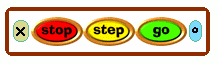
\includegraphics[scale=0.8]{Imatges/figura24-48}
\end{center}
\caption{El tauler de control d'\emph{scripts}.}
\label{fig2448}
\end{figure}
\begin{figure}[h!]
\begin{center}
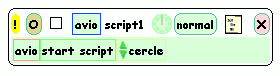
\includegraphics[scale=0.6]{Imatges/figura24-49}
\end{center}
\caption{Els mètodes \textsf{\upshape start script} i \textsf{\upshape scripting}.}
\label{fig2449}
\index{start script mètode, utilitzar a eToy}
\end{figure}

Fixeu-vos que podeu utilitzar també el mètode \textsf{start script} i el mètode relacionat \textsf{scripting} a la mateixa categoria per començar, fer una pausa o aturar \emph{scripts} (figura~\ref{fig2449}).

És interessant veure com un \emph{script} pot invocar l'execució d'altres \emph{scripts}. Això permet crear \emph{scripts} complexos.

\subsection{Eliminar}
\index{clear all pen trails mètode, utilitzar a eToy}
\index{eToy, sistema!eliminar camins dibuixats pels robots}
\index{camins dibuixats per robots, eliminar a eToy}
Podeu eliminar tots els camins dibuixats pels vostres robots amb el mètode \textsf{clear all pen trails}, a la categoria \textsf{pen use}. També podeu eliminar les traces dels jugadors des de l'escriptori. Per a això, utilitzeu la darrera opció del menú \textbf{appearance}, que podeu obtenir del menú \textbf{World}.

\subsection{Crear una icona}
\index{eToy, sistema!crear icones a|(}
\index{move toward mètode, utilitzar a eToy|(}
\index{objectes!vincular dins d'eToy|(}
\index{icona, crear dins d'eToy}
Si voleu escriure un \emph{script} que vinculi dos objectes, necessitareu referir-vos a aquests objectes. En aquest cas, us cal una \emph{icona} (\emph{tile}) que representi l'objecte a vincular per a que pugueu deixar-la anar sobre el vostre \emph{script}. Per exemple. Suposeu que teniu dos avions, un de blau i un altre de vermell, i voleu que l'avió vermell segueixi l'avió blau. Per fer això, podeu utilitzar el mètode \textsf{move toward}, mostrat a la figura~\ref{fig2450}.\index{eToy, sistema!vincular objectes}
\begin{figure}[h!]
\begin{center}
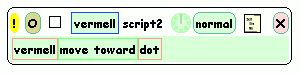
\includegraphics[scale=0.6]{Imatges/figura24-50}
\end{center}
\caption{El mètode \textsf{\upshape move toward}.}
\label{fig2450}
\end{figure}

Com que voleu que l'avió vermell es mogui cap a l'avió blau, i no cap a un \textsf{dot} com a l'\emph{script} anterior, primer utilitzeu la nansa taronja de l'avió blau per aconseguir una icona que el representi (figura~\ref{fig2451}).\index{avió!fer una icona}
\begin{figure}[h!]
\begin{center}
\includegraphics[scale=0.8]{Imatges/figura24-51}
\end{center}
\caption{Una icona que representa l'avió blau.}
\label{fig2451}
\end{figure}

Després deixeu anar aquesta icona dins de l'\emph{script}. Ara l'avió vermell segueix l'avió blau, com es pot veure a la figura~\ref{fig2452}.\index{eToy, sistema!crear icones a|)}
\begin{figure}[h!]
\begin{center}
\includegraphics[scale=0.6]{Imatges/figura24-52}
\end{center}
\caption{El tauler de control d'\emph{scripts}: l'avió vermell segueix l'avió blau.}
\label{fig2452}
\end{figure}

\subsection{Internacionalització}
\index{objectes!vincular dins d'eToy|)}
\index{move toward mètode, utilitzar a eToy|)}
\index{eToy, sistema!personalitzar|)}
\index{eToy, sistema!internacionalització}
\index{internacionalització, implementar a eToy}
\index{idiomes, tria a eToy}
Si voleu utilitzar eToy amb nens petits, voldreu que tot aparegui en la seva llengua materna. L'interfície completa d'Squeak ha estat traduïda a uns quants idiomes. Obriu el menú \textbf{World} i trieu l'opció \textbf{help\dots} seguida de \textbf{set language\dots} (figura~\ref{fig2453}). \index{set language\dots menú, mostrar a eToy}
\begin{figure}[h!]
\begin{center}
\includegraphics[scale=2]{Imatges/figura24-53i54}
\end{center}
\caption{\emph{Esquerra}: El menú per triar idioma.
\emph{Dreta}: Triar l'espanyol.}
\label{fig2453}
\end{figure}

\section{Resum}

Aquest capítol ha presentat una petita mostra de les moltes possibilitats oferides per eToy. Us suggerim que visiteu \textsf{http://www.squeakland.org} i exploreu el material que hi podreu trobar.

\chapter{Un Recorregut per Alice}
\label{cap25}
\index{Alice, entorn de creació personalitzada!accedir}
\index{Alice, entorn de creació personalitzada!propietats de}
Alice és un entorn per construir mons 3D en Squeak. Alice és també un projecte de recerca l'objectiu del qual és proporcionar un entorn prou abstracte, fàcil d'aprendre i d'utilitzar per principiants. Squeak Alice és una versió d'Alice per a Squeak feta per Jeff Pierce. Podeu trobar una descripció detallada del sistema en un dels capítols del llibre \emph{Squeak: Open Personal Computing and Multimedia}\footnote{Mark J. Guzdial i Kimberly M. Rose, \emph{Squeak: Open Personal Computing and Multimedia} (Prentice Hall, 2001).}. Squeak Alice està construït sobre \textsf{Balloon}, el motor 3D d'Squeak, que funciona en qualsevol plataforma, sense requeriments especials de maquinari. Aquest capítol presenta Squeak Alice, però dins el context d'aquest llibre.

Squeak Alice ve amb un entorn complet per manipular objectes 3D. Per desenvolupar \emph{scripts} i interactuar amb objectes 3D, podeu crear un entorn nou, com explicarem després en aquest capítol, o utilitzar l'entorn que es proporciona per defecte dins l'entorn Squeak. Per començar de pressa, us suggerim que utilitzeu primer l'entorn ja definit. Després, podeu obrir i utilitzar els vostres caràcters 3D. Aquesta és l'estratègia que seguirem en aquest capítol.

\section{Començar amb Alice} 
\index{Alice, entorn de creació personalitzada|seealso{\emph{Wonderland}}}
Quan comenceu a utilitzar un entorn Squeak estàndard, apareix una finestra anomenada \emph{The Worlds of Squeak}\footnote{\emph{Nota del Traductor:} Això passava quan es va escriure aquest llibre, als voltants de 2005. La versió actual d'Squeak, la 3.9 quan estic escrivint això, ja no té aquesta finestra inicial. Podeu, però, utilitzar versions anteriors d'Squeak, la 3.6 per exemple, si voleu jugar amb el que s'explica en aquest capítol. Les podeu trobar a \textsf{http://ftp.squeak.org}}, com veieu a la figura~\ref{fig2501}. Si feu clic en aquesta finestra, anireu a parar a un lloc que conté diverses finestres petites. Cada una d'aquestes finestres representa una demostració d'algun aspecte d'Squeak. \index{Worlds of@\emph{The Worlds of Squeak} finestra, mostrar}
\begin{figure}[h!]
\begin{center}
\includegraphics[scale=2]{Imatges/figura25-1}
\end{center}
\caption{Hi ha diversos entorns per jugar amb les característiques multimèdia d'Squeak.}
\label{fig2501}
\end{figure}

Si feu clic a la finestra anomenada 3D, arribareu a l'entorn Squeak Alice que ve donat dins d'Squeak, com veieu a la figura~\ref{fig2502}. Hi ha quatre finestres a l'escriptori: la subfinestra superior dreta és una finestra que conté algunes anotacions que ens indiquen on trobar els objectes 3D i altra informació. La subfinestra superior esquerra, que conté un conill en 3D, és el món 3D en què els objectes 3D, anomenats actors, evolucionen. La subfinestra inferior dreta és l'editor d'\emph{scripts} d'Squeak Alice. Aquesta és la finestra que farem servir per crear objectes 3D i definir \emph{scripts} per controlar aquests objectes. L'editor d'\emph{scripts} ja conté una llarga llista d'\emph{scripts} interessants que us suggerirem de provar després. La subfinestra inferior esquerra mostra una llista jeràrquica de tots els actors que existeixen actualment al món 3D.\index{Alice, entorn de creació personalitzada!mostrar per pantalla}
\begin{figure}[h!]
\begin{center}
\includegraphics[scale=0.5]{Imatges/figura25-2}
\end{center}
\caption{L'entorn Squeak Alice tal com ve definit.}
\label{fig2502}
\end{figure}

Abans que comenceu, us suggerim que comproveu la pantalla per veure quina profunditat de color hi ha definida al vostre entorn. La profunditat de color representa el nombre de colors que teniu disponibles. Per canviar-la, seleccioneu \textbf{appearance\dots} al menú \emph{World} i després \textbf{set display depth\dots} Us recomanem que proveu l'opció 32, però el resultat pot dependre de les capacitats de les vostres targetes gràfiques. Quan la profunditat de color triada no és la de la targeta gràfica, Squeak ha de transformar sempre la renderització dels objectes 3D, de manera que Alice va més lent. Un cop heu triat la profunditat de color, us suggerim que feu una mica més gran la finestra esquerra amb l'opció de la nansa groga de l'halo. Fixeu-vos que la finestra completa és anomenada ``\emph{camera}'' quan feu aparèixer l'halo; això és perque aquesta finestra mostra el que una càmera observaria al món 3D.\index{profunditat de color, comprovar i modificar}

\section{Interactuar directament amb els actors}
\index{actors a Alice!estructura jeràrquica}
\index{actors a Alice!interactuar directament amb|(}
\index{Alice, entorn de creació personalitzada!interactuant amb els actors|(}
\index{conill!moure a Alice}
Amb Squeak Alice podeu interactuar directament amb els objectes 3D, com el conill, que existeixen al món 3D:
\begin{itemize}
\item Per moure un actor horitzontalment, feu clic al món 3D. Això us permet portar el conill més lluny o més a prop dins del món.
\item Per moure verticalment un actor, premeu \textsf{Shift + Clic} (veieu la figura~\ref{fig2503}, esquerra).
\item Per girar verticalment un actor, premeu \textsf{Ctrl + Clic} (veieu la figura~\ref{fig2503}, mig).
\item Per girar lliurement un actor, premeu \textsf{Shift + Ctrl + Clic} (veieu la figura~\ref{fig2503}, dreta).
\end{itemize}
\begin{figure}[h!]
\begin{center}
\includegraphics[scale=2]{Imatges/figura25-3}
\end{center}
\caption{Podeu moure el conill amunt i avall (\emph{Shift + Clic}), girar-lo verticalment (\emph{Ctrl + Clic}), i girar-lo lliurement (\emph{Shift + Ctrl + Clic}).}
\label{fig2503}
\end{figure}

Fixeu-vos que si voleu que un actor retorni a una posició estable, utilitzeu el mètode \textsf{standUp}. Això és molt útil per experimentar amb accions realitzades en paral·lel.\index{standUp mètode, aplicar a actors dins Alice}

També podeu interactuar amb els actors via la llista dels actors disponible dins del món, com es veu a les figures~\ref{fig2504} i també~\ref{fig2502}. La llista conté tots els actors. Podeu veure que la llum, la càmera i el terra són tots actors. Podeu aplicar als actors determinades accions ja definides, com fer-los créixer, fer-los més petits, estrènyer-los, tot seleccionant l'actor i obtenint el menú emergent (figura~\ref{fig2504}, dreta).
\begin{figure}[h!]
\begin{center}
\includegraphics[scale=2.5]{Imatges/figura25-4}
\end{center}
\caption{Una llista dels actors i la seva estructura jeràrquica.}
\label{fig2504}
\end{figure}

Els actors es componen d'altres objectes. Les parts d'un actor estan estructurades jeràrquicament. Per exemple, el conill està compost d'un cap i un cos. El cap està compost d'ulleres i orelles. Les parts apareixen també a la llista, i també hi podeu realitzar accions a sobre. La figura~\ref{fig2505} mostra el conill després de la transformació següent: hem fet més petit el tambor, hem fet més gran el cap i hem tallat l'orella esquerra.\index{conill!transformar dins Alice}
\begin{figure}[h!]
\begin{center}
\includegraphics[scale=0.65]{Imatges/figura25-5}
\end{center}
\caption{Un conill transformat.}
\label{fig2505}
\end{figure}

\section{L'entorn}
\index{Alice, entorn de creació personalitzada!components|(}
\index{Alice, entorn de creació personalitzada!editor d'\emph{scripts}}
\index{actors a Alice!interactuar directament amb|)}
\index{Alice, entorn de creació personalitzada!interactuant amb els actors|)}Com ja hem mencionat, l'entorn està format principalment de tres components gràfics: l'escena, o finestra de càmera, que mostra el món 3D (finestra superior esquerra a la figura~\ref{fig2502}); la llista d'actors (figura~\ref{fig2504}); i l'editor d'\emph{scripts} (l'àrea a la dreta de la llista d'actors a la figura~\ref{fig2502}). Ara discutirem l'editor d'\emph{scripts} en detall. Hi ha tres botons al capdamunt: \textbf{Script}, \textbf{Actor Info} i \textbf{Quick Reference} (veure figura~\ref{fig2506}).
\begin{figure}[h!]
\begin{center}
\includegraphics[scale=0.5]{Imatges/figura25-6}
\end{center}
\caption{L'editor d'\emph{scripts}.}
\label{fig2506}
\index{editor d'\emph{scripts} a Alice, propietats del}
\end{figure}
\index{Actor Info (botó) a l'editor d'\emph{scripts} d'Alice}
\index{actors a Alice!mostrar informació}
\begin{itemize}
\item El botó \textbf{Script} us permet editar i executar \emph{scripts}
\item El botó \textbf{Actor Info} mostra informació relacionada amb l'actor seleccionat a la llista d'actors (figura~\ref{fig2507}).
\item El botó \textbf{Quick Reference} llista totes les accions possibles i constants definides per defecte per a cada tipus d'acció. Aquest és un ajut força útil i fàcilment accessible. \index{Quick Reference, botó dins l'editor d'\emph{scripts} d'Alice; descripció de}
\end{itemize}

Quan el botó \textbf{Script} està seleccionat, podeu definir \emph{scripts} i executar-los amb l'acció típica \textbf{do it} del menú, o bé amb \textsf{Command + D} o \textsf{Alt + D}. De fet, l'editor d'\emph{scripts} és un \emph{workspace} ampliat dedicat a l'execució d'Alice. Aquest \emph{workspace} ampliat conté variables ja definides, tal i com s'explica a la \textbf{Quick Reference}. Per a la nostra exploració heu de saber només que \textsf{camera} es refereix a la càmera per defecte, \textsf{cameraWindow} al \emph{morph} de l'escena, i \textsf{w} al \emph{Wonderland}, és a dir, el sistema Alice complet.

Fixeu-vos que Squeak Alice s'executa sense acceleració del maquinari, que està desactivat per defecte. Com a tal, Squeak Alice s'executa en qualsevol plataforma. Si voleu activar l'acceleració del maquinari, feu aparèixer el menú (nansa vermella) sobre el \emph{morph} de la càmera i seleccioneu l'opció amb l'original nom de \textbf{hardware acceleration}.
\begin{figure}[h!]
\begin{center}
\includegraphics[scale=0.5]{Imatges/figura25-7}
\end{center}
\caption{Informació dels actors.}
\label{fig2507}
\end{figure}
\index{Alice, entorn de creació personalitzada!components|)}

\section{\emph{Scripts}}
\index{Alice, entorn de creació personalitzada!utilització d'\emph{scripts}|(}
\index{scripts@\emph{scripts}!utilitzar dins d'Alice|(}
Abans de continuar, obriu els controls de la càmera, com mostrem a l'\emph{Script}~\ref{scr25-1}. D'aquesta manera, podreu seguir l'actor si és present dins l'angle de visió.
\newpage
\begin{script}  Afegir els controls de la càmera.
\textsf{\upshape
\begin{tabbing}
\hspace{5mm} \= \kill
cameraWindow showCameraControls
\end{tabbing}}
\label{scr25-1}
\end{script}

Podeu moure la càmera fent clic sobre el giny mostrat a la figura~\ref{fig2508}. Fixeu-vos que podeu moure la càmera amunt i avall apretant la tecla \textsf{Shift} mentre moveu el ratolí a sobre del giny \textsf{cameraControls}. Si per accident premeu el botó \textsf{reset} i no voleu tornar a arrencar el sistema, podeu carregar el conill com expliquem a la secció ``El Vostre Propi \emph{Wonderland}'' d'aquest capítol.\index{controls de càmera, afegint i movent a Alice}
\begin{figure}[h!]
\begin{center}
\includegraphics[scale=2]{Imatges/figura25-8}
\end{center}
\caption{Afegint els controls de càmera amb \textsf{\upshape cameraWindow showCameraControls}.}
\label{fig2508}
\end{figure}

\subsection{Analitzar el primer \emph{script}}
\index{scripts@\emph{scripts}!analitzar a Alice}
Per poder compondre accions i canviar la seva velocitat d'execució, els autors d'Alice van alterar el model d'execució de missatges. El model d'execució dels actors és diferent del que hem vist fins ara a la resta del llibre. Fins i tot si la sintaxi és la mateixa, múltiples missatges enviats a un actor no s'executen en seqüència, sinó que s'executen combinats. Compareu les diferents execucions de l'\emph{Script}~\ref{scr25-2} que obteniu executant-lo línia per línia, o executant-lo tot de cop. \index{Alice, entorn de creació personalitzada!executar missatges}
\begin{script}  Algunes accions senzilles.
\textsf{\upshape
\begin{tabbing}
\hspace{5mm} \= \kill
bunny move: forward.\\
bunny turn: left.\\
bunny move: back.\\
bunny roll: left.
\end{tabbing}}
\label{scr25-2}
\end{script}

Per executar un \emph{script} format per una seqüència d'accions, utilitzeu el mètode \textsf{doInOrder:}, com veieu a l'\emph{Script}~\ref{scr25-3}.
\begin{script}  Executar una seqüència de missatges un darrera l'altre. \index{accions!component a Alice}
\textsf{\upshape
\begin{tabbing}
\hspace{5mm} \= \kill
w doInOrder: \{ \\
\> bunny move: forward.\\
\> bunny turn: left.\\
\> bunny move: back.\\
\> bunny roll: left. \}
\end{tabbing}}
\label{scr25-3}
\end{script}

Com veieu, la diferència entre tots els efectes succeint a l'hora i succeint en seqüència és força important. Un altre aspecte important és que l'entorn \emph{Wonderland} proporciona algunes constants definides per programar actors, com per exemple \textsf{left}, \textsf{back} i \textsf{forward}, que han estat utilitzades dins l'\emph{Script}~\ref{scr25-3}. Aquí teniu una llista d'algunes de les constants disponibles pel moviment, tal i com es presenten a la subfinestra \emph{Quick Reference}. No farem servir accions relacionades amb la localització en aquest capítol. \index{Alice, entorn de creació personalitzada!compondre accions} \index{constants pel moviment a Alice, exemples de} \index{missatges!executar, a Alice}

\begin{itemize}
\item direcció: \textsf{left}, \textsf{right}, \textsf{up}, \textsf{down}, \textsf{forward} i \textsf{back}.
\item duració: \textsf{rightNow} i \textsf{eachFrame}
\item estil: \textsf{gently}, \textsf{abruptly}, \textsf{beginGently} i \textsf{endGently}
\item posició: \textsf{asIs}
\item localització: \textsf{onTopOf}, \textsf{below}, \textsf{beneath}, \textsf{inFrontOf}, \textsf{inBackOf}, \textsf{behind}, \textsf{toLeftOf}, \textsf{toRightOf}, \textsf{onFloorOf} i \textsf{onCeilingOf} 
\end{itemize}

Aquestes constants s'utilitzen per especificar variacions dels mètodes per manipular actors. LLegiu la \emph{Quick Reference} per veure les combinacions possibles.\index{moviment|seealso{robots en moviment}}

\subsection{Moure, girar i rodar}
\index{accions!crear a Alice}
\index{actors a Alice!moure, girar i rodar|(}
\index{Alice, entorn de creació personalitzada!moure, girar i rodar|(}
\index{moviment!a Alice|(}
\index{rodar a Alice, panorama general|(}
\index{turn: mètode!utilitzar dins Alice|(}
\index{girar dins Alice, panorama general|(}
\index{move: mètode, utilitzar a Alice|(}
\index{speed: mètode, utilitzar a Alice}
Els actors poden ser manipulats per moure's, girar i rodar utilitzant els mètodes \textsf{move:}, \textsf{turn:} i \textsf{roll:}, com veieu a l'\emph{Script}~\ref{scr25-3}. La subfinestra \emph{Quick Reference} mostra que aquests mètodes poden ser parametritzats per donar resultats diversos. Aqui teniu alguns exemples, però us suggerim que llegiu el capítol sobre Alice al llibre que hem esmentat al principi d'aquest capítol i la \emph{Quick Reference} per aprendre totes les possibilitats. Fixeu-vos que hi ha algunes inconsistències entre la descripció i la implementació, per tant no dubteu a experimentar. \index{distància!especificar a Alice} \index{duració, especificar pels actors a Alice}

L'\emph{Script}~\ref{scr25-4} presenta la llista tal i com es presenta a la \emph{Quick Reference}.
\begin{script}  Variacions sobre \textsf{\upshape move:}
\textsf{\upshape
\begin{tabbing}
\hspace{5mm} \= \kill
move: aDirection\\
move: aDirection distance: aNumber\\
move: aDirection distance: aNumber\\
move: aDirection distance: aNumber duration: aNumber\\
move: aDirection distance: aNumber duration: aNumber style: aStyle\\
move: aDirection asSeenBy: anActor\\
move: aDirection distance: aNumber asSeenBy: anActor\\
move: aDirection distance: aNumber duration: aNumber asSeenBy: anActor\\
move: aDirection distance: aNumber duration: aNumber asSeenBy: anActor style: aStyle\\
\\
move: aDirection speed: aNumber\\
move: aDirection speed: aNumber for: aNumber\\
move: aDirection speed: aNumber until: aBlock\\
move: aDirection speed: aNumber asSeenBy: anActor\\
move: aDirection speed: aNumber asSeenBy: anActor for: aNumber\\
move: aDirection speed: aNumber asSeenBy: anActor until: aBlock
\end{tabbing}}
\label{scr25-4}
\end{script}

Aquí teniu algunes explicacions: Primer, podeu especificar una \emph{distància} utilitzant \textsf{distance:}. Després hauríeu de saber que, per defecte, una animació triga un segon en executar-se. Per canviar aquest comportament per defecte podeu especificar una altra \emph{duració} amb \textsf{duration:} i donar el nombre de segons que l'animació hauria de durar. De fet, fins i tot si definiu una duració de zero, pot no ser executat instantàniament pel \emph{Wonderland}. Si realment voleu animacions instantànies, utilitzeu la constant \textsf{rightNow}. També podeu especificar un \emph{estil}, utilitzant \textsf{style:} i les constants associades \textsf{gently}, \textsf{abruptly}, \textsf{beginGently} i \textsf{endGently} que descriuen com hauria de començar o acabar l'animació. \index{Alice, entorn de creació personalitzada!aturar animacions} \index{animacions!aturar, dins d'Alice} \index{until: mètode; utilitzar a Alice}

Les accions són normalment depenents del temps, la qual cosa vol dir que tenen un començament i un final. També podeu crear accions persistents, amb \textsf{speed:}, que especifica que els actors s'haurien de moure a una velocitat constant. Pareu atenció que si utilitzeu \textsf{speed:} però ometeu la distància, l'actor es mourà per sempre. L'argument de velocitat pel mètode \textsf{move:} són metres per segon, mentre que pel mètode \textsf{turn:} és el nombre de girs per segon. L'argument especificat per \textsf{for:} us permet especificar una duració per al missatge quan utilitzeu velocitat; \textsf{until:} us permet especificar una condició, expressada mitjançant un bloc, que determinarà si l'acció continua. Fixeu-vos que podeu aturar l'animació amb el missatge \textsf{stop}.\index{for: mètode; utilitzar a Alice}

Per defecte, accions com \textsf{move:} i \textsf{turn:} prenen com a referència l'actor mateix. Per tant, quan dieu \textsf{bunny turn: left} el conill girarà cap a la seva esquerra. De vegades voldreu especificar algun altre marc de referència, i en aquest cas hauríeu d'utilitzar \textsf{asSeenBy:} que us permet especificar un altre marc de referència, com veieu als exemples de l'\emph{Script}~\ref{scr25-5}.\index{missatges!variacions a Alice}
\begin{script}  Exemples de variacions sobre missatges.
\textsf{\upshape
\begin{tabbing}
\hspace{5mm} \= \kill
bunny move: forward distance: 3 duration: rightNow style: endGently\\
bunny move: forward distance: 3 duration: 0\\
bunny move: forward distance: 3 duration: rightNow\\
bunny move: forward distance: 5 speed: 1\\
bunny move: left distance: 3 duration: 3 asSeenBy: camera\\
bunny turn: left turns: 3 speed: 1\\
bunny roll: right turns: 2
\end{tabbing}}
\label{scr25-5}
\end{script}
\index{actors a Alice!moure, girar i rodar|)} \index{Alice, entorn de creació personalitzada!moure, girar i rodar|)} \index{moviment!a Alice|)} \index{turn: mètode!utilitzar dins Alice|)}

\section{Parts dels actors}
\index{actors a Alice!parts de|(}
\index{rodar a Alice, panorama general|)}
\index{animacions!crear parts independents per a}
\index{Alice, entorn de creació personalitzada!utilització d'\emph{scripts}|)}
\index{girar dins Alice, panorama general|)}
\index{scripts@\emph{scripts}!utilitzar dins d'Alice|)}
\index{move: mètode, utilitzar a Alice|)}
Els actors estan formats per parts en una relació jeràrquica pare-fill. Les parts pertanyen només a un sol progenitor. Aquesta relació és important ja que les accions enviades a un actor afecten les seves parts. Per exemple, quan demaneu al conill que mogui el cap, les ulleres, que formen part del cap, també es mouen. Les parts no són res d'especial. Senzillament són actors als quals podeu enviar missatges, com il·lustrem a l'\emph{Script}~\ref{scr25-6}.
\begin{script}  Enviar missatges a parts.
\textsf{\upshape
\begin{tabbing}
\hspace{5mm} \= \kill
bunny drum roll: left bunny drum roll: left speed: 1\\
\\
w doInOrder: \{\\
\> bunny head glasses move: forward.\\
\> bunny head glasses move: back \}\\
\\
bunny drum stop
\end{tabbing}}
\label{scr25-6}
\end{script}

De fet, tots els actors són parts d'un super-progenitor anomenat l'\emph{escena} (\emph{scene}). Si observeu la llista jeràrquica que mostra tots els actors del Món, veieu l'escena, i a sota, amb sagnat, el conill, però també el terra, el llum i la càmera. \index{Alice, entorn de creació personalitzada!variacions de missatges} \index{missatges!enviar parts dels actors, a Alice|(}

De vegades necessiteu enviar un missatge a un objecte afectant només algunes de les seves parts. Per exemple, voleu canviar el color del conill sense canviar el color de la seva orella esquerra; així doncs, heu de fer l'orella independent de la resta del conill. Per fer això, Alice introdueix la noció d'objecte de \emph{primera classe}. Una part de \emph{primera classe} pertany al progenitor però no es veu afectada per canvis al progenitor. A la figura~\ref{fig2509} podeu veure com hem separat el cap del conill de la resta. \index{Alice, entorn de creació personalitzada!objectes de primera classe} \index{primera classe, objectes de; descripció a Alice|(}
\begin{figure}[h!]
\begin{center}
\includegraphics[scale=0.65]{Imatges/figura25-9}
\end{center}
\caption{Un cos independent per fer dibuixos animats.}
\label{fig2509}
\end{figure}

Dos mètodes us permeten controlar si un objecte és part d'un altre. El mètode \textsf{becomeFirstClass} fa que el receptor es torni un objecte de primera classe, mentre el mètode \textsf{becomePart} fa que el receptor sigui part del seu progenitor. Executeu l'\emph{Script}~\ref{scr25-7} línia a línia per entendre la diferència.\index{objectes!manipular dins d'Alice}
\begin{script}  Exemples de parts de primera classe.
\textsf{\upshape
\begin{tabbing}
\hspace{5mm} \= \kill
bunny setColor: green.\\
bunny head becomeFirstClass.\\
bunny setColor: red.\\
bunny head becomePart.\\
bunny setColor: pink
\end{tabbing}}
\label{scr25-7}
\end{script}

També podeu canviar la relació progenitor-fill entre objectes utilitzant el mètode \textsf{becomeChildOf} (veieu l'\emph{Script}~\ref{scr25-8}).\index{actors a Alice!parts de|)} \index{Alice, entorn de creació personalitzada!canviar la relació progenitor-fill dels objectes} \index{primera classe, objectes de; descripció a Alice|)}
\newpage
\begin{script}  Enviar missatges a parts.
\textsf{\upshape
\begin{tabbing}
\hspace{5mm} \= \kill
bunny head becomeChildOf: ground\\
bunny move: forward\\
ground head turn: left
\end{tabbing}}
\label{scr25-8}
\end{script}

\section{Altres operacions}
\index{missatges!enviar parts dels actors, a Alice|)}
Els actors entenen molts més missatges del que us hem ensenyat fins ara. Aquí teniu una descripció senzilla dels altres mètodes.

\subsection{Fer-se gran}
\index{resize: mètode, utilitzar dins Alice|(}
\index{Alice, entorn de creació personalitzada!canviar de mida els receptors|(}
El mètode \textsf{resize:} canvia la mida del receptor. Existeix en moltes variacions, com \textsf{resize:duration:}, \textsf{resizeTopToBottom:leftToRight:frontToBack:}, i \textsf{resizeLikeRubber:dimension:}, com veieu a l'\emph{Script}~\ref{scr25-9}.
\begin{script}  Experiments canviant la mida.
\textsf{\upshape
\begin{tabbing}
\hspace{5mm} \= \kill
bunny resize: 1/2\\
bunny resizeTopToBottom: 2 leftToRight: 1 frontToBack: 3\\
bunny resizeLikeRubber: 2 dimension: topToBottom
\end{tabbing}}
\label{scr25-9}
\end{script}

\subsection{Moviments quantificats}
\index{resize: mètode, utilitzar dins Alice|)}
\index{Alice, entorn de creació personalitzada!canviar de mida els receptors|)}
\index{Alice, entorn de creació personalitzada!utilització del mètode nudge}
\index{nudge: mètode, utilitzar a Alice}
El mètode \textsf{nudge:} mou un actor en múltiples de la seva longitud, amplada o alçada en funció de la direcció triada.
\begin{script}  Experiments amb \textsf{\upshape nudge:}.
\textsf{\upshape
\begin{tabbing}
\hspace{5mm} \= \kill
bunny nudge: up distance: 2 duration: 2
\end{tabbing}}
\label{scr25-10}
\end{script}

\subsection{Mantenir-se dret}
\index{Alice, entorn de creació personalitzada!utilització dels mètodes standUp}
Els mètodes \textsf{standUp} i \textsf{standUpWithDuration: unNombre} permeten que un actor es mogui a una posició vertical, la qual cosa pot ser útil després de fer experiments.

\subsection{Acolorir}
\index{Alice, entorn de creació personalitzada!utilització del mètode setColor:}
\index{setColor: mètode, utilitzar a Alice}
El mètode \textsf{setColor:} canvia el color del receptor. Existeix de maneres molt variades, com \textsf{setColor:duration:} i \textsf{setColor:duration:style:}. Fixeu-vos en l'\emph{Script}~\ref{scr25-7} per veure un exemple.

\subsection{Destrucció}
\index{Alice, entorn de creació personalitzada!utilització del mètode destroy}
\index{destroy mètode a Alice, utilitzar}
El mètode \textsf{destroy} destrueix un actor amb una animació divertida. Afortunadament, l'entorn \emph{Wonderland} té un mecanisme potent per desfer (\emph{undo}) accions.

\subsection{Visibilitat}
\index{Alice, entorn de creació personalitzada!utilització dels mètodes hide i show}
Els mètodes \textsf{hide} i \textsf{show} gestionen la visibilitat d'un objecte.\index{hide i show mètodes a Alice, utilitzar}

\subsection{Moviments absoluts i rotacions}
\index{moveTo: i move: mètodes a Alice, utilitzar|(}
\index{Alice, entorn de creació personalitzada!utilització dels mètodes moveTo: i move:|(}
Fins ara hem utilitzat només accions que canvien la posició o la direcció d'un actor. El mètode \textsf{moveTo:} mou el receptor a un lloc donat, i el mètode \textsf{turnTo:} fa que el receptor apunti a una posició determinada. La posició i la direcció poden ser un triplet de la forma \textsf{\{ dreta . amunt . endavant \}} o bé \textsf{unActor}. Els valors del triplet poden ser nombres o bé \textsf{asIs} (per exemple, \textsf{\{ asIs . 0 . asIs \}}). Fixeu-vos que el triplet descriu una posició al marc de referència del progenitor de l'actor. Per tant \textsf{bunny moveTo: \{ 1 . 1 . 0 \}} significa que el conill s'hauria de moure 1 metre a la dreta i 1 metre per sobre de l'origen de l'escena, que és el progenitor de l'actor conill. El mateix triplet a l'expressió \textsf{bunny head moveTo: \{ 1 . 1 . 0 \}} es refereix a la posició 1 metre a la dreta i 1 metre per sobre de la posició origen del conill.

Compareu les accions de \textsf{moveTo:} i de \textsf{move:} a l'\emph{Script}~\ref{scr25-11}.
\begin{script}  Experiments amb moviments absoluts
\textsf{\upshape
\begin{tabbing}
\hspace{5mm} \= \kill
bunny moveTo: \{0 . 0 . 0\}.\\
bunny head moveTo: \{0 . 1 . 0\}.\\
bunny head moveTo: \{0 . -1 . 0\}\\
bunny head move: up.\\
bunny head move: down\\
bunny head turnTo: camera duration: 1 style: abruptly\\
bunny turnTo: camera duration: 1 style: abruptly
\end{tabbing}}
\label{scr25-11}
\end{script}

Fixeu-vos que el mètode \textsf{alignWith: unActor} és equivalent a \textsf{turnTo:}\index{moveTo: i move: mètodes a Alice, utilitzar|)}

\subsection{Apuntar}
\index{Alice, entorn de creació personalitzada!utilització dels mètodes moveTo: i move:|)}
\index{Alice, entorn de creació personalitzada!utilització del mètode pointAt:}
\index{pointAt: mètode d'Alice}
El mètode \textsf{pointAt: unObjectiu} permet que els actors es vegin entre ells. Un objectiu pot ser un actor, un moviment \textsf{\{ dreta . amunt . endavant \}} o una posició de píxel \textsf{x@y}.
\newpage
\begin{script}  Experiments amb \textsf{\upshape pointAt:}.
\textsf{\upshape
\begin{tabbing}
\hspace{5mm} \= \kill
bunny pointAt: camera.\\
bunny turn: left.\\
bunny move: forward.\\
camera pointAt: bunny.
\end{tabbing}}
\label{scr25-12}
\end{script}

\subsection{Posicionament relatiu dels actors.}
\index{Alice, entorn de creació personalitzada!utilització del mètode place:}
\index{place: mètode a Alice, utilitzar}
\index{actors a Alice!posicionament relatiu}
Finalment, els actors poden ser col·locats en posicions relatives respecte d'altres actors, utilitzant el mètode \textsf{place: unLloc object: unActor}. Les posicions s'especifiquen amb les constants \textsf{onTopOf}, \textsf{below}, \textsf{beneath}, \textsf{inFrontOf}, \textsf{inBackOf}, \textsf{behind}, \textsf{toLeftOf}, \textsf{toRightOf}, \textsf{onFloorOf} i \textsf{onCeilingOf}. Proveu de carregar molts actors, tal i com explicarem més tard, i jugueu amb les expressions de l'\emph{Script}~\ref{scr25-13}.
\begin{script}  Col·locar els actors.
\textsf{\upshape
\begin{tabbing}
\hspace{5mm} \= \kill
camera place: inFrontOf object: bunny.\\
camera move: up.\\
bunny move: back distance: 2.\\
camera pointAt: bunny.\\
bunny head place: toRightOf object: bunny
\end{tabbing}}
\label{scr25-13}
\end{script}

\section{Accions relacionades amb el temps}
\index{Alice, entorn de creació personalitzada!accions relacionades amb el temps|(}
\index{accions relacionades amb el temps, definir a Alice|(}
També podeu definir accions que es relacionen amb el pas del temps utilitzant la constant \textsf{eachFrame} com a argument de \textsf{duration:}, com podeu veure a l'\emph{Script}~\ref{scr25-14}. Utilitzeu el mètode \textsf{stop} per aturar l'animació (veieu la propera secció).
\begin{script}  Utilitzar la constant \textsf{\upshape eachFrame}.
\textsf{\upshape
\begin{tabbing}
\hspace{5mm} \= \kill
bunny head pointAt: camera duration: eachFrame.\\
bunny move: forward
\end{tabbing}}
\label{scr25-14}
\end{script}

També podeu especificar la durada d'una acció en segons quan l'acció utilitza l'opció \textsf{eachFrameFor: unNombre}, com en l'\emph{Script}~\ref{scr25-15}. \index{durada d'una acció, especificar a Alice} \index{Alice, entorn de creació personalitzada!especificant la durada d'una acció}
\begin{script}  Restringir una acció una determinada durada.
\textsf{\upshape
\begin{tabbing}
\hspace{5mm} \= \kill
bunny moveTo: \{asIs . 0 . asIs\} eachFrameFor: 10
\end{tabbing}}
\label{scr25-15}
\end{script}

El mètode \textsf{eachFrameFor: unNombre} fa que les accions es repeteixin un cert nombre de segons. El mètode \textsf{eachFrameUntil: unBloc} repeteix les accions fins que el bloc retorna \textsf{true}. \index{eachFrame constant, utilitzar a Alice}

Fixeu-vos que \textsf{asIs} és una constant especial que manifesta que el mètode executat no modificarà el valor actual. Deixa el valor ``tal com està'' (``\emph{as is}''). Altres mètodes, però, poden canviar aquest valor. Aquí l'\emph{script} restringeix el conill a seguir el terreny. Fixeu-vos també que el triplet significa \textsf{\{ dreta . amunt . endavant \}} i per tant el conill no es pot moure amunt o avall per un període de 10 segons.\index{asIs constant, utilitzar a Alice}

\section{Animació}
\index{Alice, entorn de creació personalitzada!definir animacions|(}
\index{Alice, entorn de creació personalitzada!accions relacionades amb el temps|)}
\index{accions relacionades amb el temps, definir a Alice|)}
\index{animacions!definir dins d'Alice|(}
Per definir una animació, només cal assignar-la a una variable. Per exemple, declarem a l'\emph{Script}~\ref{scr25-16} que \textsf{spin} fa girar dues vegades el conill cap a l'esquerra durant 2 segons.
\begin{script}  Una animació senzilla.
\textsf{\upshape
\begin{tabbing}
\hspace{5mm} \= \kill
spin := bunny turn: left turns: 2 duration: 2.
\end{tabbing}}
\label{scr25-16}
\end{script}

Podeu aturar temporalment l'animació (\textsf{spin pause}), tornar a posar-la en marxa (\textsf{spin resume}), aturar-la del tot (\textsf{spin stop}) o començar-la altre cop (\textsf{spin start}).

Les animacions també poden repetir-se utilitzant els mètodes \textsf{loop} i \textsf{loop: unNombreDeRepeticions}, o aturar les repeticions amb \textsf{stopLooping}.
\begin{script}  Una animació senzilla
\textsf{\upshape
\begin{tabbing}
\hspace{5mm} \= \kill
flip := bunny turn: forward turns: 1 duration: 2.
\end{tabbing}}
\label{scr25-17}
\end{script}

Ara podeu compondre animacions amb el mètode \textsf{doInOrder:}, que executa una seqüència de missatges en seqüència, o \textsf{doTogether:}, que executa una seqüència de missatges combinant-los.
\begin{script}  Dues animacions senzilles executades en seqüència.
\textsf{\upshape
\begin{tabbing}
\hspace{5mm} \= \kill
w doInOrder: \{spin start . flip loop:2\}
\end{tabbing}}
\label{scr25-18}
\end{script}

\begin{script}  Dues animacions senzilles compostes.
\textsf{\upshape
\begin{tabbing}
\hspace{5mm} \= \kill
w doTogether: \{spin start . flip loop:2\}
\end{tabbing}}
\label{scr25-19}
\end{script}

Fixeu-vos que hi ha combinacions que no funcionen i us podeu trobar amb un \emph{walkback} (una finestra que us notifica que hi ha un problema). Una composició pot rebre un nom i formar part d'altres animacions.
\begin{script}  Dues animacions senzilles compostes en seqüència.
\textsf{\upshape
\begin{tabbing}
\hspace{5mm} \= \kill
bla := w doInOrder: \{spin start . flip loop:2\}. bla start
\end{tabbing}}
\label{scr25-20}
\end{script}

Recordeu que el mètode \textsf{standUp} fa que l'actor romangui vertical de peu, la qual cosa és útil després de resultats inesperats en compondre accions.\index{Alice, entorn de creació personalitzada!definir animacions|)}

\section{El vostre propi \emph{Wonderland}}
\index{Wonderland@\emph{Wonderland}!crear dins Alice|(}
\index{Alice, entorn de creació personalitzada!crear \emph{Wonderland}|(}
\index{animacions!definir dins d'Alice|)}
Podeu crear el vostre propi \emph{Wonderland} executant l'\emph{Script}~\ref{scr25-21}.
\begin{script}  Obrir un nou \emph{Wonderland}.
\textsf{\upshape
\begin{tabbing}
\hspace{5mm} \= \kill
Wonderland new
\end{tabbing}}
\label{scr25-21}
\end{script}

Un cop hagueu creat el vostre propi \emph{Wonderland}, o després de prémer el botó de \emph{reset}, hauríeu de carregar alguns objectes 3D. L'equip que desenvolupa Alice proporciona un fitxer ZIP ple de personatges 3D a \textsf{http://www.cs.cmu.edu/$\sim$jpierce/squeak/SqueakObjects.zip} (o busqueu-los a \textsf{http://www.apress.com}). Aquests objectes es representen en un format antic, i per tant provar de carregar els nous objectes Alice no funcionarà a Squeak.

Podeu crear un avió senzill, com a simple experiment, amb l'expressió \textsf{w makePlaneNamed: 'avioMeu'}. Aquí teniu com carregar objectes 3D en un PC (\emph{Script}~\ref{scr25-22}) o en Mac OS X (\emph{Script}~\ref{scr25-23}). \index{w makePlaneNamed: expressió; utilitzar a Alice}
\begin{script}  Carregar nous objectes 3D en un PC.
\textsf{\upshape
\begin{tabbing}
\hspace{5mm} \= \kill
w makeActorFrom: 'Objects{\textbackslash}Animals{\textbackslash}Bunny.mdl'
\end{tabbing}}
\label{scr25-22}
\end{script}

\begin{script}  Carregar nous objectes 3D en Mac OS X.
\textsf{\upshape
\begin{tabbing}
\hspace{5mm} \= \kill
w makeActorFrom: ':Objects:Animals:PurpleDinosaur.mdl'\\
\\
``si teniu problemes al mac utilitzeu el nom complet''\\
w makeActorFrom: 'OSX:Users:ducasse:Alice:Objects:Animals:PurpleDinosaur.mdl'
\end{tabbing}}
\label{scr25-23}
\end{script}

Després de carregar diversos personatges, com el ninot de nou o el dinosaure porpra (figura~\ref{fig2510}), podeu escriure i executar els \emph{Scripts}~\ref{scr25-24} i~\ref{scr25-25}.
\newpage
\begin{figure}[h!]
\begin{center}
\includegraphics[scale=0.5]{Imatges/figura25-10}
\end{center}
\caption{Els tres amics.}
\label{fig2510}
\end{figure}

\begin{script}  \emph{Script} amb diversos actors.
\textsf{\upshape
\begin{tabbing}
\hspace{5mm} \= \kill
bunny turn: left\\
bunny turn: left asSeenBy: snowman\\
snowman place: inFrontOf object: purpleDinosaur.
\end{tabbing}}
\label{scr25-24}
\end{script}

\begin{script}  Una mirada ràpida al conill.
\textsf{\upshape
\begin{tabbing}
\hspace{5mm} \= \kill
w doInOrder: \{\\
\> purpleDinosaur head pointAt: bunny\\
\> purpleDinosaur head alignWith: purpleDinosaur \}
\end{tabbing}}
\label{scr25-25}
\end{script}

\section{Múltiples càmeres i altres efectes especials}
\index{Wonderland@\emph{Wonderland}!crear dins Alice|)}
\index{efectes especials, utilitzar a Alice}
\index{controls de càmera, afegint i movent a Alice|(}
\index{conill!script@\emph{script} de mostra}
\index{script@\emph{script} amb diversos actors a Alice, exemple de}
\index{Alice, entorn de creació personalitzada!múltiples càmeres|(}
\index{Alice, entorn de creació personalitzada!crear \emph{Wonderland}|)}
\index{Alice, entorn de creació personalitzada!efectes especials|(}
Tenir diverses càmeres pot fer que la renderització 3D d'Alice sigui més lenta, però val la pena entendre com funciona per construir animacions. Quan es crea una nova càmera, també es crea una nova visualització. Igual que un objecte 3D nou que representa la càmera. Canviar la localització de la càmera fent clic a sobre automàticament canvia la visualització que mostra allò que veu la càmera. A més, canviar la posició de la càmera utilitzant el giny dels controls de la càmera modifica la posició de l'objecte càmera.

A la figura~\ref{fig2511}, hi ha tres càmeres. Hem triat la càmera de la dreta per tenir una visió panoràmica de l'escena, mentre que les dues càmeres de l'esquerra s'han situat per proporcionar diferents plans propers del conill. L'\emph{Script}~\ref{scr25-26} mostra com afegir una altra finestra de càmera.

\begin{script}  Crear una altra finestra de càmera.
\textsf{\upshape
\begin{tabbing}
\hspace{5mm} \= \kill
w makeCamera
\end{tabbing}}
\label{scr25-26}
\end{script}

Fixeu-vos que una càmera és un actor com qualsevol altre objecte 3D, i per tant el podeu moure utiltzant els missatges mostrats a l'\emph{Script}~\ref{scr25-27}.\index{controls de càmera, afegint i movent a Alice|)}

\begin{script}  Moure una càmera.
\textsf{\upshape
\begin{tabbing}
\hspace{5mm} \= \kill
w doInOrder: \{\\
\> camera roll: left.\\
\> camera move: back distance: 4.\\
\> camera standUp.\}
\end{tabbing}}
\label{scr25-27}
\end{script}

\begin{figure}[h!]
\begin{center}
\includegraphics[scale=0.5]{Imatges/figura25-11}
\end{center}
\caption{Les finestres de l'esquerra mostren el que les càmeres de la finestra de la dreta veuen.}
\label{fig2511}
\end{figure}

\section{Alarmes}
\index{Wonderland@\emph{Wonderland}|seealso{Alice, entorn de creació personalitzada}}
\index{Wonderland@\emph{Wonderland}!alarmes}
\index{Alice, entorn de creació personalitzada!múltiples càmeres|)}
\index{Alice, entorn de creació personalitzada!efectes especials|)}
\index{alarma, programar dins un \emph{Wonderland}}
Cada \emph{Wonderland} manté un seguiment del temps gràcies a un objecte planificador de tasques (\emph{scheduler}). Quan es crea un \emph{Wonderland}, es posa el comptador de temps a zero, i el planificador comença a actualitzar aquest comptador de temps a cada marc. Podeu obtenir el temps actual utilitzant l'expressió \textsf{scheduler getTime}. El que és interessant és que podeu programar una \emph{alarma} per executar certes accions en un moment determinat utilitzant el mètode \textsf{do:at:inScheduler:}, o, un cop ha passat un determinat període de temps, utilitzant el mètode \textsf{do:in:inScheduler:}. L'\emph{Script}~\ref{scr25-28} defineix dues alarmes. \index{scheduler getTime expressió, utilitzar dins \emph{Wonderland}} \index{temps!conèixer dins del \emph{Wonderland} a Alice}

\begin{script}  Dues alarmes.
\textsf{\upshape
\begin{tabbing}
\hspace{5mm} \= \hspace{5mm} \= \kill
Alarm\\
\> do:\\
\>\> [ bunny head turn: left turns: 3.\\
\>\> bunny setColor: red ]\\
\> at: (scheduler getTime + 5)\\
\> inScheduler: scheduler.\\
\\
Alarm\\
\> do: [bunny setColor: pink]\\
\> in: 8\\
\> inScheduler: scheduler.
\end{tabbing}}
\label{scr25-28}
\end{script}

Podeu enviar els següents missatges a una alarma: \textsf{checkTime}, que retorna el temps en què l'alarma s'hauria d'executar, i \textsf{stop}, que aturarà l'alarma si encara no s'ha executat del tot. \index{Alice, entorn de creació personalitzada!aconseguint el temps per \emph{Wonderland}}


\section{Introduir la interacció amb l'usuari}
\index{accions!definir a Alice}
\index{usuari, interacció amb; implementar dins Alice|(}
\index{addResponse:to: i respondWith:to: mètodes a Alice, comparar}
\index{Alice, entorn de creació personalitzada!eliminar accions|(}
\index{Alice, entorn de creació personalitzada!interacció amb l'usuari|(}
En aquest moment podeu programar animacions, però encara no podeu definir interaccions amb l'usuari. Squeak Alice us permet vincular accions als actors quan succeeixen determinats esdeveniments, com els clics del ratolí. Per exemple, l'\emph{Script}~\ref{scr25-29} fa que el conill giri el cap quan fem clic al damunt amb el botó dret del ratolí.

\begin{script}  Definir una acció associada amb un clic del botó dret del ratolí.
\textsf{\upshape
\begin{tabbing}
\hspace{5mm} \= \kill
bunny respondWith: [:event | bunny head turn: left turns: 1] to: rightMouseClick
\end{tabbing}}
\label{scr25-29}
\end{script}

Els tres mètodes \textsf{addResponse: unBloc to: tipusEsdeveniment}, \textsf{removeResponse: unBloc to: tipusEsdeveniment} i \textsf{respondWith: unBloc to: tipusEsdeveniment} gestionen la definició de les accions. Les accions s'expressen utilitzant blocs i s'associen amb tipus d'esdeveniments, entre els quals podem trobar els següents: \textsf{keyPress}, \textsf{leftMouseDown}, \textsf{leftMouseDown}, \textsf{leftMouseClick}, \textsf{rightMouseDown}, \textsf{rightMouseUp} i \textsf{rightMouseClick}.

La diferència entre els mètodes \textsf{addResponse:to:} i \textsf{respondWith:to:} és que el primer us permet definir diverses accions associades al mateix tipus d'esdeveniment, mentre que el segon elimina les accions prèviament definides i en defineix una de nova. El mètode \textsf{removeResponse:to:} elimina les accions corresponents. Un exemple utilitzant \textsf{removeResponse:to:} apareix a l'\emph{Script}~\ref{scr25-30}. \index{accions!eliminar a Alice}
\begin{script}  Definir una acció associada amb un clic del botó esquerre del ratolí.
\textsf{\upshape
\begin{tabbing}
\hspace{5mm} \= \hspace{5mm} \= \kill
bunny\\
respondWith:\\
\> [:event $|$\\
\> bunny head turn: left turns: 2 duration: 2.\\
\> w doInOrder: \{\\
\>\> bunny head move: up.\\
\>\> bunny head move: down\}] to: leftMouseClick
\end{tabbing}}
\label{scr25-30}
\end{script}

A l'\emph{Script}~\ref{scr25-31} hem afegit dues reaccions i després hem eliminat la primera de manera que només s'executa la segona quan feu clic a sobre del conill.
\begin{script}  Gestionar les respostes.
\textsf{\upshape
\begin{tabbing}
\hspace{5mm} \= \hspace{5mm} \= \kill
reaction := bunny\\
\> addResponse: [ :event $|$ bunny head turn: left turns: 1 ]\\
\> to: rightMouseClick.\\
bunny\\
\> addResponse: [ :event $|$ bunny head pointTo: \{ 0 . 0 . 0 \} ]\\
\> to: rightMouseClick.\\
bunny removeResponse: reaction to: rightMouseClick
\end{tabbing}}
\index{reaccions, tractant-les dins Alice}
\label{scr25-31}
\end{script}

\section{Aspectes ocults d'Alice i Pooh}
\index{usuari, interacció amb; implementar dins Alice|)}
\index{Alice, entorn de creació personalitzada!eliminar accions|)}
\index{Alice, entorn de creació personalitzada!interacció amb l'usuari|)}
Ens agradaria acabar aquesta presentació d'Squeak Alice mostrant-vos alguns aspectes divertits que il·lustren també la potència d'Alice.

\subsection{Projectar \emph{morphs} 2D en 3D}
\index{Alice, entorn de creació personalitzada!projectar \emph{morphs} 2D en 3D|(}
Podeu posar \emph{morphs} 2D en objectes 3D. El procés és el següent:
\begin{itemize}
\item Primer feu aparèixer la nansa vermella \textbf{menu} a la finestra de la càmera i seleccioneu l'opció \textbf{accept drops}, com veieu a la figura~\ref{fig2512}.
\begin{figure}[h!]
\begin{center}
\includegraphics[scale=0.65]{Imatges/figura25-12}
\end{center}
\caption{\emph{Esquerra:} El conill abans.
\emph{Dreta:} Diem a la càmera que accepti objectes deixats anar sobre el conill}
\label{fig2512}
\end{figure}
\item Després creeu un \emph{morph} actiu; per exemple, feu aparèixer la finestra dels objectes utilitzant l'opció \textbf{objects (o)}, o \textsf{Command + Q}, del menú principal d'Squeak i creeu un \emph{morph} d'àtoms que reboten com veieu a la figura~\ref{fig2513}.\index{morphs@\emph{morphs}, crear a Alice}
\begin{figure}[h!]
\begin{center}
\includegraphics[scale=0.5]{Imatges/figura25-13}
\end{center}
\caption{\emph{Esquerra:} La finestra dels objectes.
\emph{Mig:} Un \emph{morph} d'àtoms que reboten.
\emph{Dreta:} Un \emph{morph} actiu projectat sobre un objecte 3D.}
\label{fig2513}
\end{figure}
\item Deixeu anar el \emph{morph} que acabeu de crear sobre alguna part del conill. Usualment, el \emph{morph} s'hauria de projectar a l'objecte 3D, com veieu a la figura~\ref{fig2513} (dreta).
\end{itemize}

Finalment, l'\emph{Script}~\ref{scr25-32} mostra un aspecte divertit i potent d'Alice i Squeak. Crea un mur a través del que podeu veure el que està apuntant el ratolí.
\begin{script}  Diversió amb Alice.
\textsf{\upshape
\begin{tabbing}
\hspace{5mm} \= \hspace{5mm} \= \kill
w makePlaneNamed: 'test'.\\
test\\
doEachFrame:\\
\> [ test setTexturePointer:\\
\>\> (Form fromDisplay: ((Sensor mousePoint) extent: 50@50)) asTexture ]
\end{tabbing}}
\label{scr25-32}
\end{script}
\index{Alice, entorn de creació personalitzada!projectar \emph{morphs} 2D en 3D|)}
\section{Pooh: generar formes 3D a partir de 2D}
\index{Wonderland@\emph{Wonderland}!obrir per utilitzar amb Pooh}
\index{Pooh, generar formes 3D a partir de figures 2D amb el sistema|(}
\index{Alice, entorn de creació personalitzada!utilització d'eToy amb}
Pooh és un sistema que us permet generar formes 3D dibuixant formes 2D dins d'un món Alice. Si teniu curiositat, proveu de fer el següent:
\begin{itemize}
\item Obriu un nou món \emph{Wonderland} (\textsf{Wonderland new}).
\item Feu aparèixer l'halo de la finestra de la càmera, com veieu a la figura~\ref{fig2514}
\begin{figure}[h!]
\begin{center}
\includegraphics[scale=0.5]{Imatges/figura25-14}
\end{center}
\caption{Obrir l'halo de la càmera d'Alice per obtenir accés a Pooh}
\label{fig2514}
\end{figure}
\item Seleccioneu l'halo blanc del mig a la dreta amb la icona petita de l'ós.
\item Dibuixeu una corba tancada directament a la finestra de la càmera. Quan acabeu, Pooh genera una forma 3D, com podeu veure a la figura~\ref{fig2515} (dreta)
\begin{figure}[h!]
\begin{center}
\includegraphics[scale=1.25]{Imatges/figura25-15}
\end{center}
\caption{\emph{Esquerra:} Obtenir una forma 3D.
\emph{Dreta:} Obtenir l'editor de dibuixos sobre una forma 3D.}
\label{fig2515}
\end{figure}
\item Ara podeu dibuixar dins la forma obtenint l'halo de la nova forma i triant la nansa del llapis que teniu al centre, com podeu veure a la figura~\ref{fig2515}. Això obre un editor de dibuixos. Quan acabeu, premeu el botó \emph{Keep} de l'editor de dibuixos. La figura~\ref{fig2516} mostra la foma anterior dibuixada. També mostra que podeu girar aquesta forma, i qualsevol altre.
\begin{figure}[h!]
\begin{center}
\includegraphics[scale=1.25]{Imatges/figura25-16}
\end{center}
\caption{\emph{Esquerra:} Una vaca dibuixada.
\emph{Dreta:} La mateixa vaca girada.}
\label{fig2516}
\end{figure}
\end{itemize}

Finalment ens agradaria mostrar-vos alguns aspectes experimentals d'Squeak. Podeu utilitzar eToy, presentat en el capítol anterior, amb els objectes 3D d'Alice. Podeu obtenir un visualitzador amb la nansa de l'ull de l'objecte 3D utilitzant les mateixes tècniques que vam explicar al capítol~\ref{cap24}. La figura~\ref{fig2517} mostra un senzill \emph{script}.\index{eToy, sistema!utilitzar amb objectes 3D a Alice}\index{Pooh, generar formes 3D a partir de figures 2D amb el sistema|)}
\begin{figure}[h!]
\begin{center}
\includegraphics[scale=0.5]{Imatges/figura25-17}
\end{center}
\caption{Utilitzar un \emph{script} eToy per controlar un objecte 3D.}
\label{fig2517}
\end{figure}

\section{Resum}

Alice és un entorn molt potent. Us hem mostrat només uns quants dels aspectes més importants. El lector interessat hauria de llegir el capítol dedicat a Alice dins del llibre sobre Squeak mencionat al començament d'aquest capítol.


